%\motto{Use the template \emph{chapter.tex} to style the various elements of your chapter content.}
\chapter{Fehlerkorrektur}
\label{error_correction} % Always give a unique label
% use \chaptermark{}
% to alter or adjust the chapter heading in the running head

\chapterauthor{Niklas Bodfeld, Tim Boschert, Manuel Meixner, Ann-Kathrin Wenzel}

\abstract{}Quantencomputer versprechen enorme Rechenvorteile, sind jedoch hochgradig fehleranfällig. Das Kapitel analysiert systematisch die in Quantenrechnern auftretenden Fehlertypen, von physikalischen Störquellen über hardwarebedingte Grenzen bis zur Modellierung und Auswirkung auf Algorithmen und Architektur. Darauf aufbauend werden zentrale Prinzipien der Quantenfehlerkorrektur vorgestellt: Fehlererkennung ohne Zustandsmessung, redundante Informationsverteilung, Unterscheidbarkeit und reversible Korrektur von Fehlern, lokale Fehlerbegrenzung sowie das Fehlerschwellenprinzip. Anschließend werden praktische Realisierungen skizziert, insbesondere der Fehlerkorrekturzyklus von Oberflächencodes, aktuelle technische Hürden und künftige Perspektiven. Den Abschluss bildet ein praxisnahes Beispiel anhand des Shor-Codes inklusive Implementierung in IBM Qiskit, das die theoretischen Konzepte in eine konkrete Anwendung überführt.

\section{Fehlertypen in Quantenrechnern}\label{chap:QEC1}
\subsection{Die Herausforderung von Fehlern in Quantencomputern}
 Ein zentrales Hindernis bei der praktischen Realisierung von Quantencomputern ist die Fehleranfälligkeit. Diese treten in Quantensystemen häufiger auf als in klassischen Rechnern und sind viel schwerer zu kontrollieren.
Während klassische Systeme mit extrem niedrigen Fehlerraten arbeiten (unter $10^{-17}$), liegen diese bei heutigen Quantenprozessoren um Größenordnungen zwischen $10^{-3}$ und $10^{-1}$. Der Grund dafür liegt unter anderem in der hohen Empfindlichkeit von Qubits gegenüber Umwelteinflüssen wie elektromagnetischen Feldern, Temperaturfluktuationen oder Strahlungen. Hinzu kommen Fehler durch ungenaue Hardware, Crosstalk zwischen benachbarten Qubits und unzuverlässige Mess- oder Initialisierungsprozesse. vgl.\cite[Seite 48-49]{tutschke_quantencomputing_2023}\medskip

Quantenfehler sind ein Zusammenspiel aus unvermeidbaren physikalischen Prozessen, technologischen Grenzen und Umwelteinflüssen. Sie zu verstehen und zu kontrollieren, ist eine der größten Herausforderungen beim Bau und Betrieb eines funktionierenden Quantencomputers. Die Auswirkungen dieser Fehler sind tiefgreifend. Schon ein einzelner Fehler kann sich durch Verschränkung auf das gesamte System ausbreiten. Besonders kritisch sind Phasenfehler, da sie die Interferenzmuster zerstören können, auf denen viele Quantenalgorithmen beruhen.
Physikalische Ursachen von Fehlern im Quantencomputing wirken direkt auf die empfindlichen Quantenzustände der Qubits ein. Diese physikalischen Einflüsse führen zu konkreten Fehlertypen. Welche dieser Fehlerarten in der Praxis überwiegt, hängt maßgeblich von der jeweiligen Hardwareplattform ab. So sind beispielsweise supraleitende Qubits besonders anfällig für Defasierungseffekte, während bei Ionenfallen Laserstabilität eine große Rolle spielt. Die Art und Weise, wie physikalische Effekte in konkrete Fehler münden, ist also eng mit den technischen Eigenschaften und Grenzen der verwendeten Hardware verbunden.
Aus gegebenen Gründen ist die Entwicklung effektiver Fehlerkorrekturmethoden ein zentrales Thema für die Zukunft des Quantencomputings. Nur wenn bestimmte Mechanismen greifen, kann der theoretische Nutzen in der Praxis ausgeschöpft werden.


\subsection{Physikalische Fehlerursachen in Quantenrechnern}
Quantencomputer arbeiten nicht mit Bits sondern mit Qubits, die sich gleichzeitig in mehreren Zuständen befinden können. Die quantenmechanischen Eigenschaften von Qubits, insbesondere die Superposition, ermöglichen das enorme Potenzial und die Leistungsstärke von Quantencomputern. Gleichzeitig machen sie Quantencomputer allerdings auch extrem empfindlich. Schon geringe äußere Einflüsse können die Zustände stören und zu Fehlern führen. Im Folgenden werden zentrale physikalische Ursachen näher betrachtet.\medskip


\textbf{Dekohärenz}

Da sich physikalische Qubits nicht vollständig von ihrer Umgebung isolieren lassen, kommt es durch unvermeidliche Wechselwirkungen zu Dekohärenz, einem zentralen Fehlermechanismus in der Quanteninformatik.
Dekohärenz beschreibt den Prozess, bei dem ein Qubit durch den Kontakt mit seiner Umgebung „gestört“ wird und dabei seine Fähigkeit verliert, sich in einem Überlagerungszustand zu befinden. Stattdessen verhält es sich zunehmend wie ein klassisches Bit. Das bedeutet, dass die Quanteninformation, die zuvor im Zustand des Qubits gespeichert war, verloren geht. Anders als klassische Fehler entsteht Dekohärenz nicht durch eine fehlerhafte Bedienung oder ungenaue Operationen, sondern ist ein grundlegendes physikalisches Phänomen, das automatisch auftritt, sobald ein Quantensystem mit seiner Umgebung interagiert.

Es wird dabei zwischen Phasendekohärenz und Amplitudendekohärenz unterschieden. Bei der Phasendekohärenz bleibt das Qubit formal im selben Zustand, also zum Beispiel in $|0\rangle$ oder $|1\rangle$, jedoch verändert sich die relative Phase zwischen diesen Zuständen. Diese Phase ist zentral für Quanteninterferenz, einem Grundprinzip, das es Quantencomputern ermöglicht, durch Überlagerung unterschiedliche Rechenwege effizient zu nutzen. Wird die Phase gestört, kann der Quantencomputer falsche oder keine sinnvollen Ergebnisse mehr liefern. 

Amplitudendekohärenz hingegen beschreibt einen echten Energieverlust des Qubits. Wenn es aus einem angeregten Zustand $|1\rangle$ in den Grundzustand $|0\rangle$ zurückfällt. Solche Prozesse treten unter anderem durch spontane Emission oder Wärmeaustausch mit der Umgebung auf und sind in physischen Systemen wie supraleitenden Qubits oder Ionenfallen besonders häufig zu beobachten.

Die Wirkung solcher Umweltkopplungen lässt sich mathematisch mithilfe der sogenannten Operator-Summen-Zerlegung (Kraus-Zerlegung) beschreiben. Die Zerlegung erlaubt es, die Störung eines Qubits durch die Umgebung als Wahrscheinlichkeitsmischung mehrerer Fehlerprozesse darzustellen. Dies ist entscheidend für die Entwicklung von Quantenfehlerkorrektur und bildet die theoretische Grundlage für den Umgang mit Umwelteinflüssen.

Ein häufig verwendetes Modell zur Beschreibung solcher Fehler ist das lokale und Markov’sche Fehlermodell. Es geht davon aus, dass jedes Qubit nur mit seiner eigenen lokalen Umgebung interagiert (lokal) und dass sich diese Umgebung bei jedem Zeitschritt erneuert bzw. unabhängig vom Zustand in vorherigen Zeitintervallen ist (Markov). Die Gesamtwirkung auf ein Mehr-Qubit-System lässt sich dann als Produkt von Einzeleffekten auf die jeweiligen Qubits darstellen. Dieses Modell ist realistisch und erlaubt es, die meisten heute verwendeten Quantenfehlerkorrekturverfahren zu formulieren. 

Insgesamt zeigt sich, dass Dekohärenz  ein unvermeidlicher, aber mathematisch gut beschreibbarer Effekt ist. Durch geeignete Fehlerkorrektur und die Annahme realistischer Fehlermodelle kann ihre Auswirkung auf Quanteninformationen deutlich reduziert werden. vgl. \cite[Seite 332-339]{rieffelQuantumComputingGentle2011a}\medskip



\textbf{Rauschen und Vibration}

Doch Dekohärenz ist nicht die einzige physikalische Fehlerursache in Quantencomputern. Weitere Ursachen liegen in verschiedenen Rauschprozessen. Das sind zufällige oder unkontrollierte Störungen aus der Umgebung. Dazu zählen unter anderem thermisches Rauschen, das durch Temperaturunterschiede entsteht, sowie elektromagnetische Fluktuationen, verursacht durch Stromleitungen, elektronische Geräte oder sogar Mobilfunkstrahlung. Auch mechanische Vibrationen stellen eine Störquelle dar. Diese können beispielsweise durch Pumpen oder Bewegungen im Kühlapparat ausgelöst werden und sich auf die empfindlichen Qubits übertragen. In Systemen wie Ionenfallen können solche Vibrationen die Bewegung der Ionen stören. Dies führt dazu, dass die Quantenobjekte ihre Überlagerungszustände verlieren und sich zunehmend klassisch verhalten. Gleichzeitig wirken zufällige elektrische Feldschwankungen auf die Teilchen, wodurch es zu unkontrollierten Energie- und Positionsänderungen kommen kann. Wird dabei das harmonische Potenzial gestört, verlassen die Ionen ihren quantenmechanischen Grundzustand, was zu Rechenfehlern führt. Besonders problematisch wird dies bei stark gekoppelten Qubits, bei denen viele Operationen wie CNOT-Gatter notwendig sind. Denn jede zusätzliche Operation erhöht die Anfälligkeit für Rauschen und überfordert in vielen Fällen die heutigen Fehlermitigationstechniken. Um diese Fehler zu minimieren, sind hochstabile Betriebsbedingungen sowie gezielte Kühl- und Isolationsmaßnahmen unerlässlich. vgl. \cite[Seite 39-43]{tutschke_quantencomputing_2023}; \cite[Seite 353-356]{nielsen_quantum_2010}\medskip



\textbf{Unvollständige Isolation}

Ein besonderes Problem ist die unzureichende Isolation der Qubits. Idealerweise sollte ein Qubit vollständig von seiner Umgebung abgeschottet sein. In der Realität ist das fast nicht möglich. Selbst im Vakuum oder bei extrem tiefen Temperaturen gibt es noch mikroskopisch kleine Wechselwirkungen mit anderen Teilchen, Materialien oder Defekten. Manche Materialien enthalten zum Beispiel sogenannte Zwei-Niveau-Systeme, die mit den Qubits interagieren können und als zusätzliche Störquellen wirken. Auch kosmische Strahlung oder Magnetfelder aus der Umgebung können Störungen verursachen.

Aus all diesen Gründen ist es extrem wichtig, die Quantenhardware so gut wie möglich gegen äußere Einflüsse zu schützen. Das geschieht zum Beispiel durch ultratiefe Temperaturen im Millikelvin-Bereich, durch spezielle Abschirmungen gegen elektromagnetische Wellen, durch mechanische Entkopplung der Geräte und durch den Einsatz besonders reiner Materialien ohne Defekte. Trotzdem lässt sich nie ganz vermeiden, dass äußere Einflüsse auf das System wirken. Daher ist es bedeutend, zusätzlich auf softwareseitige Verfahren zur Fehlerkorrektur zu setzen. vgl. \cite[Seite 24-26]{tutschke_quantencomputing_2023}



\subsection{Klassifizierung von Quantenfehlern}\label{chap:QEC1.3}
Die Klassifikation von Quantenfehlern stellt eine bedeutsame Grundlage für die Entwicklung stabiler Fehlerkorrekturverfahren im Quantencomputing dar. Aufgrund der Superposition können Fehler nicht nur den Zustand selbst, sondern auch die relative Phase, Amplitude oder die Kohärenzeigenschaften eines Qubits beeinflussen. Die Einteilung unterscheidet zwischen diskreten, kontinuierlichen, zufälligen und systematischen Fehlern.

Die diskreten Fehlerarten sind die Pauli-Fehler. Die einfachste und zugleich mathematisch fundamentale Klasse von Quantenfehlern basiert auf den sogenannten Pauli-Fehlern, benannt nach den drei Pauli-Matrizen 
X, Y und Z. Diese Operatoren stellen Basisoperationen im zweidimensionalen Qubit-Zustandsraum dar und bilden eine vollständige Fehlerbasis für beliebige Ein-Qubit-Störungen.\medskip



\textbf{Bit-Flip-Fehler (X-Fehler)}

Ein Bit-Flip-Fehler ist eine der einfachsten und grundlegendsten Fehlerarten in der Quanteninformatik. Er beschreibt eine Umkehrung des Zustands eines Qubits, also einen Wechsel von $|0\rangle$ nach $|1\rangle$ oder von $|1\rangle$ nach $|0\rangle$. Formal wird dieser Fehler durch den X-Operator (auch Pauli-X-Gatter genannt) dargestellt, der wie ein klassisches NOT-Gatter wirkt: X$|0\rangle$=$|1\rangle$, X$|1\rangle$=$|0\rangle$. Ein solcher Fehler kann in der physikalischen Realität zum Beispiel durch thermische Anregung entstehen. Also wenn ein Qubit spontan aus dem Grundzustand $|0\rangle$ in einen angeregten Zustand $|1\rangle$ übergeht, weil es mit seiner Umgebung Energie austauscht.

Beim Bit-Flip-Fehler geht es also ausschließlich um die Veränderung der Besetzungszustände eines Qubits, nicht um seine Phase oder Superposition. Er ist die quantenmechanische Entsprechung eines klassischen Bitfehlers, bei dem eine „0“ zu einer „1“ wird oder umgekehrt. vgl. \cite[Seite 246-251]{rieffelQuantumComputingGentle2011a}\medskip



\textbf{Phase-Flip-Fehler (Z-Fehler)}

Ein Phase-Flip-Fehler (auch Z-Fehler) ist eine fundamentale Art von Fehler in der Quanteninformationstheorie, die nicht den Zustand $|0\rangle$ oder $|1\rangle$ selbst verändert, sondern die relative Phase zwischen ihnen. Formal wird dieser Fehler durch den Z-Operator (Pauli-Z-Gatter) dargestellt: $Z|0\rangle$=$|0\rangle$,$Z|1\rangle$=$-|1\rangle$. Obwohl sich der Zustand $|1\rangle$ dabei nicht in $|0\rangle$ umwandelt, bekommt er ein negatives Vorzeichen. Die sogenannte Phaseninversion. Für Zustände wie $|0\rangle$ oder $|1\rangle$ alleine ist dieser Effekt nicht direkt sichtbar. Doch sobald der Qubit-Zustand eine Superposition ist, wirkt sich der Fehler messbar aus. Besonders deutlich wird das in diesem Zustand: \[
|+\rangle = \frac{1}{\sqrt{2}}(|0\rangle + |1\rangle)
\]
Wird darauf der Z-Operator angewendet, entsteht:
\[
Z|+\rangle = \frac{1}{\sqrt{2}}(|0\rangle - |1\rangle) = |-\rangle
\]

Damit wird die Phase zwischen den beiden Zustandsanteilen vertauscht. Das hat gravierende Folgen für Quantenalgorithmen, die auf Interferenz und kohärenter Phasenevolution beruhen. Phase-Flip-Fehler stören also genau diese empfindlichen quantenmechanischen Effekte, die Quantencomputer leistungsfähig machen. vgl. \cite[Seite 251-252]{rieffelQuantumComputingGentle2011a}\medskip



\textbf{Kombinierte Bit- und Phase-Fehler (Y-Fehler)}

Der Y-Operator kombiniert Bit- und Phase-Flip in einem einzigen Fehler: Y=iXZ. Er wirkt gleichzeitig wie ein X- (Bit-Flip) und ein Z-Operator (Phase-Flip) und ist damit der vollständigste Einzelfehler im Pauli-Basisset. Solche Fehler treten typischerweise bei komplexeren physikalischen Störungen auf. Dazu zählt unter anderem Crosstalk zwischen benachbarten Qubits, Störfelder mit nichtlokaler Auswirkung oder gekoppelte Fluktuationen in Steuerleitungen. In der Fehlerkorrektur werden Y-Fehler daher als gleichzeitiges Auftreten von X- und Z-Fehlern behandelt und können entsprechend über Stabiliser-Messungen erkannt werden.

Diese drei Operatoren bilden eine vollständige Fehlerbasis für \\ Ein-Qubit-Störungen. Jeder beliebige Fehler auf einem Qubit kann mathematisch als Linearkombination von I, X, Y und Z dargestellt werden. Diese Eigenschaft ist von Bedeutung für den Aufbau von Quantenfehlerkorrekturcodes wie dem Shor-Code oder dem Steane-Code, welche gezielt auf Pauli-Fehler reagieren.  vgl. \cite[Seite 252-253]{rieffelQuantumComputingGentle2011a}\medskip



\textbf{Dämpfung}

Neben diskreten Fehlern gibt es die kontinuierlichen Fehlerprozesse, die sich über sogenannte Quantenkanäle modellieren lassen. Die zwei wichtigsten Beispiele sind Amplitudendämpfung und die Phasendämpfung. Sie hängen eng mit den physikalischen Prozessen der Phasen- und Amplitudendämpfung zusammen.

Die Amplitudendämpfung beschreibt den Verlust von Energie durch das Qubit, etwa infolge spontaner Emission oder thermischer Relaxation. Der Zustand $|1\rangle$ relaxiert dabei mit einer gewissen Wahrscheinlichkeit $\gamma$ in den Grundzustand $|0\rangle$. vgl. \cite[Seite 380-383]{nielsen_quantum_2010}

Bei der Phasendämpfung (Dephasing) geht keine Energie verloren, aber Kohärenz. Die Off-Diagonal-Elemente der Dichtematrix, also die, die Superpositionen erzeugen, werden gedämpft. Dies geschieht durch Umwelteinflüsse wie Fluktuationen elektromagnetischer Felder. In der Praxis ist Phasendämpfung oft die dominante Dekohärenzquelle. vgl. \cite[Seite 383-386]{nielsen_quantum_2010}\medskip



\textbf{Zufällige vs. Systematische Fehler}

Quantenfehler lassen sich nicht nur nach ihrer physikalischen Form, sondern auch nach ihrer Entstehungsart klassifizieren. Hierzu zählen zufällige Fehler und systematische Fehler.

Zufällige Fehler (stochastisch) entstehen unvorhersehbar durch thermisches Rauschen, Photonen-Einfälle, kosmische Strahlung oder spontane Kopplungen an die Umgebung. Sie sind oft kurzzeitig, unkorreliert und lassen sich statistisch modellieren.
Systematische Fehler beruhen auf wiederholbaren, deterministischen Einflüssen, wie falscher Kalibrierung von Pulssequenzen, ungenauen Gatterzeiten oder falsch modellierter Kopplung. Solche Fehler summieren sich über Zeit auf und können ganze Rechenprozesse verfälschen. Sie sind schwerer zu korrigieren, da sie nicht durch Mittelwertbildung „herausrauschen“. vgl. \cite[Seite 3-5]{acharyaQuantumErrorCorrection2025a}
Die Unterscheidung ist für die Architekturplanung bedeutend, da systematische Fehler oft durch verbesserte Hardware, kontrollierte Steuerungen oder modellgestützte Korrektur vermieden werden können.

Ein wachsendes Problem in größeren Quantenprozessoren ist das Auftreten von korrelierten Fehlern. Solche Fehler beeinflussen mehrere Qubits gleichzeitig und können durch gemeinsame Störquellen oder durch ungewollte Kopplungen entstehen. Anders als unabhängige Fehler breiten sie sich nicht lokal aus, sondern erzeugen komplexe Fehlerbilder, die von klassischen Fehlerkorrekturmodellen oft nicht erfasst werden.


\subsection{Hardwarebedingte Fehler und Systematische Grenzen}
Neben den oben beschriebenen Fehlern spielen auch hardwarebedingte Fehler eine zentrale Rolle in der Fehlertheorie des Quantencomputings. Diese entstehen durch Unzulänglichkeiten in der technischen Umsetzung der Steuerung, der Auslese und der physikalischen Qubit-Architektur. In realen Quantenprozessoren, wie supraleitenden Schaltkreisen, Ionenfallen oder spinbasierten Systemen, sind diese Fehlerquellen ein wesentlicher begrenzender Faktor für die Skalierbarkeit und Zuverlässigkeit der Systeme.\medskip



\textbf{Gatteroperationen}

Ein wesentliches Problem sind fehlerhafte Gatteroperationen. Idealerweise sollen Quantenlogikgatter wie das CNOT- oder Hadamard-Gate eine definierte unitäre Transformation auf den Zustand der Qubits ausführen. In der Praxis weichen die implementierten Operationen von diesem Ideal ab. Ursachen dafür sind unter anderem folgende Fehler:

\begin{itemize}
     

\item Timing-Fehler: Ungenauigkeiten in der Pulslänge oder -frequenz führen zu nicht vollständig abgeschlossenen Rotationen.
\item Crosstalk: Eine ungewollte Kopplung zwischen benachbarten Qubits oder Steuerleitungen kann zu Störungen führen, die nicht auf das Zielqubit beschränkt bleiben.
 \item Leakage-Fehler: Besonders bei supraleitenden oder mehrstufigen Systemen kann ein Qubit durch ein Gatter in höhere Energiezustände außerhalb des Rechenraums (z.B. $|2\rangle$) übergehen, was spätere Gates unbrauchbar macht.
\item Falsche Kalibrierung: Abweichungen in der Kalibrierung der Steuerpulse führen dazu, dass Operationen (z.B. ein X-Gate) nicht exakt das tun, was vorgesehen ist, etwa eine Rotation um 178° statt 180°.
\end{itemize}
Diese Gatterfehler häufen sich über tiefe Schaltkreise hinweg und führen dazu, dass die logische Fehlerrate mit zunehmender Schaltungstiefe exponentiell ansteigt. Selbst bei modernen Quantenprozessoren liegt die mittlere Gatterfidelität, also die Wahrscheinlichkeit, mit der ein Gatter korrekt ausgeführt wird, typischerweise nur bei 99–99,9 \%. vgl. \cite[Seite 2-5]{acharyaQuantumErrorCorrection2025}; \cite[Seite 5-13]{kang_timeadaptive_2025}\medskip



\textbf{Messfehler}

Ein weiterer kritischer Aspekt sind Messfehler. Die Auslese eines Qubits erfolgt in der Regel über die Verstärkung und Analyse eines quantenmechanischen Signals. Dabei können verschiedene Fehlerquellen auftreten. Zum Beispiel elektronisches Rauschen in der Verstärkerschaltung, Überlappung der Signalverteilungen für die Zustände $|0\rangle$ und $|1\rangle$ oder Verzögerungen und Sättigungseffekte in der Ausleseelektronik. Solche Störungen können dazu führen, dass der tatsächliche Zustand des Qubits falsch interpretiert wird. Dies beeinträchtigt nicht nur die Genauigkeit von Quantenalgorithmen, sondern besonders auch die Fehlerkorrektur, die auf das zuverlässige Auslesen von Syndromen angewiesen ist. vgl. \cite[Seite 49-51]{tutschke_quantencomputing_2023}; \cite[Seite 5-7]{kang_timeadaptive_2025}\medskip



\textbf{Qubitinitalisierung}

Die Initialisierung von Qubits ist ein grundlegender Schritt zu Beginn jeder Quantenberechnung. Ziel ist es, sämtliche Qubits zuverlässig in den Grundzustand $|0\rangle$ zu bringen. In der Praxis gelingt dies jedoch nicht immer mit perfekter Genauigkeit. Mögliche Ursachen sind zum Beispiel thermische Anregungen bei unzureichender Kühlung, unvollständige Relaxation aus angeregten Zuständen oder Restkopplungen an Resonatoren oder benachbarte Qubits. Fehlerhafte Initialisierungen beeinflussen unmittelbar die Ausführung der ersten Gatteroperationen und können sich über den gesamten Quantenschaltkreis hinweg auswirken. vgl. \cite[Seite 3-5]{acharyaQuantumErrorCorrection2025}\medskip



\textbf{Konnektivität}

In skalierbaren Architekturen, vor allem in zweidimensionalen Gittern supraleitender Qubits, sind nicht alle Qubits direkt miteinander verbunden. Diese eingeschränkte Konnektivität führt dazu, dass logische Operationen, die Qubits an weit entfernten Positionen betreffen, durch zusätzliche SWAP-Gatter oder Relaisoperationen realisiert werden müssen. Diese zusätzlichen Schritte erhöhen nicht nur die Rechenzeit, sondern fügen dem System zusätzliche Fehlerquellen hinzu. Besonders kritisch ist dies in tiefen Schaltkreisen oder bei komplexen Algorithmen. vgl. \cite[Seite 49-51]{tutschke_quantencomputing_2023}\medskip


\textbf{Kalibrierfehler}

Alle oben genannten Fehlerarten werden zusätzlich durch Kalibrierfehler \\verstärkt. Diese entstehen, wenn die physikalischen Parameter des Systems, wie Frequenzen, Kopplungsstärken, Pulsamplituden oder Dämpfungsraten nicht exakt bekannt oder nicht stabil sind. Selbst kleine Abweichungen in der Kalibrierung können über viele Rechenzyklen hinweg zu signifikanten Abweichungen im Endergebnis führen. Studien zeigen, dass Kalibrierfehler insbesondere bei nicht regelmäßig durchgeführten Rekalibrierungszyklen zu systematischer Fehlentwicklung der Qubit-Zustände führen. vgl. \cite[Seite 5-7]{acharyaQuantumErrorCorrection2025a}

\subsection{Quantifizierung und Modellierung von Quantenfehlern}
Die präzise Modellierung und Quantifizierung von Fehlern in Quantencomputern ist wichtig, um deren Auswirkungen auf die Informationsverarbeitung zu verstehen und wirksame Fehlerkorrekturstrategien zu entwickeln. Aufgrund der Besonderheiten quantenmechanischer Systeme, insbesondere Superposition, Nichtklassikalität und Unitarität, ist eine Beschreibung von Fehlerprozessen nur durch formalisierte mathematische Modelle möglich, die über klassische Störmodelle weit hinausgehen. In der Theorie offener Quantensysteme werden solche Fehler durch Quantenkanäle beschrieben, deren Wirkung über sogenannte Krausoperatoren modelliert wird.\medskip



\textbf{Fehlerkanäle und Krausoperatoren}

Ein Quantenkanal beschreibt die Wirkung eines Umgebungseinflusses auf ein Quantensystem, das sich dadurch in einen neuen Zustand überführt. Formal wird ein Quantenkanal (E) durch eine completely positive, trace-preserving (CPTP) Abbildung auf dem Raum der Dichtematrizen definiert. Die Wirkung eines solchen Kanals auf einen Zustand $\rho$ wird durch die Kraus-Zerlegung beschrieben:

$$
E(\rho) = \sum_k E_k \rho E_k^\dagger, \quad \text{mit} \quad \sum_k E_k^\dagger E_k = I.
$$

Hierbei sind  $E_k$ die Krausoperatoren, die jeweils eine mögliche Fehlerwirkung modellieren. Diese Darstellung ist besonders mächtig, da sie sowohl diskrete als auch kontinuierliche Fehlermechanismen integriert. Je nach Art des Rauschprozesses ergeben sich unterschiedliche konkrete Kanalformen:\medskip

Amplitudendämpfungskanal: Modelliert Energieverluste wie spontane Emission. Dabei relaxiert das Qubit mit Wahrscheinlichkeit 
$\gamma$ vom angeregten Zustand $|1\rangle$ in den Grundzustand $|0\rangle$. Die zugehörigen Krausoperatoren lauten:


$$
E_0 = \begin{pmatrix} 1 & 0 \\ 0 & \sqrt{1-\gamma} \end{pmatrix}, \quad E_1 = \begin{pmatrix} 0 & 0 \\ \sqrt{\gamma} & 0 \end{pmatrix}
$$


Depolarisationskanal: Beschreibt symmetrisches Rauschen, bei dem mit Wahrscheinlichkeit p ein zufälliger Pauli-Fehler (X, Y, Z) auftritt:

$$
\mathcal{E}(\rho) = (1-p)\rho + \frac{p}{3}(X\rho X + Y\rho Y + Z\rho Z)
$$


Diese Modelle bilden die Grundlage für theoretische Fehleranalysen und sind integraler Bestandteil moderner Simulationen von Quantenalgorithmen. vgl. \cite[Seite 379-397]{nielsen_quantum_2010}\medskip



\textbf{Fehlerraten}

Fehlerraten spielen eine zentrale Rolle bei der Quantifizierung und Modellierung von Quantenfehlern, insbesondere im Kontext der derzeit verfügbaren NISQ-Quantencomputer („Noisy Intermediate-Scale Quantum“). Diese Systeme sind durch verschiedene Störfaktoren stark limitiert. Dazu zählen kurze Kohärenzzeiten (T1 und T2), begrenzte Qubit-Konnektivität, Crosstalk und insbesondere die Fehlerraten bei Quantengattern und Messungen. Die Gate-Fidelity, also die Wahrscheinlichkeit, mit der ein Quantengatter korrekt ausgeführt wird, liegt derzeit bei etwa 0,1\% Fehler für 1-Qubit-Gatter und etwa 1\% Fehler für 2-Qubit-Gatter. Auch bei der Initialisierung und Auslesung treten mit etwa 1\% signifikante Fehler auf. Diese Fehlerraten sind um Größenordnungen höher als bei klassischen Computern und schränken die maximale Schaltungstiefe sowie die Verlässlichkeit von Quantenalgorithmen massiv ein. Um diese Fehler systematisch zu erfassen und vergleichbar zu machen, wurden Metriken wie das „Quantenvolumen“ entwickelt. Es kombiniert Aspekte wie Qubit-Anzahl, Gate-Fidelity und Schaltungstiefe zu einer einzigen Kenngröße. Allerdings ist diese Metrik nicht unumstritten, da die Aussagekraft stark vom konkreten Anwendungsfall abhängt. In jedem Fall ist eine präzise Quantifizierung und Modellierung der Fehlerraten unerlässlich, um die Einsatzfähigkeit von Quantencomputern realistisch bewerten zu können und eine effektive Fehlerkorrektur zu ermöglichen. vgl. \cite{marre_welche_2021}\medskip



\textbf{Fehlergrenzen und Fehlertolernaz}

Ein zentrales Konzept in der Quantenfehlertoleranz ist die sogenannte Fehlergrenze (Threshold). Diese beschreibt den maximal tolerierbaren physikalischen Fehler \( p \) der Qubits, unterhalb dessen ein Fehlerkorrekturcode in der Lage ist, die logische Fehlerwahrscheinlichkeit 
\( p_{L} \) 
durch Vergrößerung des Codes zu unterdrücken. Ist der physikalische Fehler kleiner als der Schwellenwert \( p_{L} \) , kann die logische Fehlerquote beliebig klein gemacht werden. Der Code wirkt also stabilisierend. Liegt der physikalische Fehler jedoch über diesem Schwellenwert, wird die Fehlerkorrektur kontraproduktiv und verschlechtert den Zustand. Für den in der Praxis besonders relevanten Surface Code liegt der theoretische Schwellenwert bei etwa 10,9\% (bei separater Behandlung von X- und Z-Fehlern). Mit realistischen Decodierungsalgorithmen liegt der praktische Schwellenwert bei etwa 10,3\%.

Ein weiterer kritischer Aspekt ist die Fehlertoleranz (Fault Tolerance) von Quantenfehlerkorrekturverfahren. Dabei geht es nicht nur darum, Fehler im Qubit-Zustand selbst zu erkennen und zu beheben, sondern auch Fehler, die während des Korrekturprozesses auftreten, beispielsweise bei Zwei-Qubit-Gates oder bei der Syndrommessung, korrekt zu behandeln. Eine fehlertolerante Fehlerkorrektur muss gewährleisten, dass sich solche Fehler nicht unkontrolliert ausbreiten. Dies wird beispielsweise durch spezielle Schaltungen, redundante Hilfsqubits (Ancillas) oder wiederholte Messungen über mehrere Zyklen erreicht. Diese zusätzlichen Anforderungen erhöhen jedoch den Ressourcenbedarf erheblich. In realistischen Szenarien, insbesondere bei Surface Codes mit fehlerhaften Syndrommessungen, reduziert sich der Schwellenwert dadurch auf etwa 1\%. Dennoch ist dieser Wert für moderne Quantenhardware erreichbar, da aktuelle Systeme bereits Fehlerquoten unterhalb dieser Grenze aufweisen. vgl. \cite[Seite 13-15]{roffe_quantum_2019} 

\subsection{Auswirkungen von Fehlern auf Quantenalgorithmen und Systemarchitektur}
Fehler haben tiefgreifende Auswirkungen auf die Funktionsweise von Quantenalgorithmen und die Gestaltung von Quantencomputer-Architekturen. Bereits kleinste Abweichungen durch Umwelteinflüsse oder ungenaue Operationen können den empfindlichen Quantenzustand stören. Solche Störungen zeichnen sich in Form von Dekohärenz, Gate-Fehlern und Messfehlern ab. Besonders kritisch ist die Dekohärenz, also der Verlust von Quantenkohärenz, die essenziell für Superpositions- und Verschränkungszustände ist. Algorithmen, die stark auf Interferenzeffekten beruhen, werden dadurch extrem fehleranfällig. Ein einzelner Fehler kann das gesamte Interferenzmuster zerstören und damit das korrekte Ergebnis verhindern. vgl. \cite[Seite 381-385]{nielsen_quantum_2010}\medskip

Diese hohe Fehleranfälligkeit wirkt sich direkt auf die algorithmische Struktur aus. Je größer die Schaltungstiefe, also die Anzahl nacheinander geschalteter Operationen, desto wahrscheinlicher treten Fehler auf. Aktuelle Hardware beschränkt die maximale Tiefe daher erheblich. Entwickler müssen daher bereits beim Entwurf von Quantenalgorithmen Strategien zur Fehlertoleranz berücksichtigen. Ein zentrales Konzept in diesem Zusammenhang ist der sogenannte Fehlerschwellenwert (Threshold), der angibt, bis zu welchem Maß an physikalischen Fehlern eine zuverlässige Fehlerkorrektur überhaupt möglich ist. vgl. \cite[Seite 293-308]{rieffelQuantumComputingGentle2011a}\medskip

Auch auf der Systemarchitektur wirkt sich die Fehleranfälligkeit massiv aus. Um fehlerhafte physikalische Qubits nutzbar zu machen, werden sie in logische Qubits zusammengefasst, die durch Fehlerkorrekturcodes geschützt sind. Dieser Schritt ist jedoch teuer. Die Anzahl der tatsächlich benötigten physikalischen Qubits steigt exponentiell mit dem Anspruch an Fehlertoleranz. Beispielsweise kann ein logisches Qubit je nach Code und Fehlerrate mehrere hundert oder tausend physikalische Qubits benötigen. vgl. \cite[Seite 435–437]{nielsen_quantum_2010}; \cite[Seite 246-253]{rieffelQuantumComputingGentle2011a}\medskip

Liegt die effektive Fehlerrate pro Gatteroperation oder Qubit unterhalb dieser Fehlerschwelle, so kann durch wiederholte Korrekturzyklen ein logisch fehlerfreier Zustand aufrechterhalten werden. Wird sie überschritten, kann auch ein noch so ausgeklügelter Fehlerkorrekturcode das System nicht mehr retten.

Die Gestaltung der Quantenhardware und -architektur muss daher darauf ausgerichtet sein, mit einer begrenzten Anzahl physikalischer Qubits möglichst effektive Fehlerresistenz zu gewährleisten. Dazu gehören unter anderen fehlertolerante Layouts, z.B. zweidimensionale Qubit-Gitter mit lokaler Nachbarschaftsstruktur, die einfache Syndrome-Messung und Korrektur ermöglichen.
Die konkrete Umsetzung solcher Codes, wie etwa des 9-Qubit Shor-Codes, zeigt, dass verschiedene Arten von Fehlern, wie der Bit-Flip, Phase-Flip und kombinierte Fehler, durch geeignete Verschränkung und Syndrommessung identifiziert und korrigiert werden können. Dies setzt jedoch eine Systemarchitektur voraus, die gezielte Paarung und Interaktion zwischen Qubits erlaubt, was hohe Anforderungen an die Qubit-Konnektivität und Kohärenz stellt.\medskip

Fehler wirken sich aber nicht nur auf die Hardware, sondern auch auf die Softwareebene aus. Quantenalgorithmen müssen so entworfen sein, dass sie entweder robust gegenüber Fehlern sind oder mit reduzierten Ressourcen für Fehlerkorrektur arbeiten. Dafür werden auch softwarebasierte Fehlermitigationstechniken verwendet, etwa die statistische Nachbearbeitung von Messergebnissen oder hybride Strategien, bei denen klassische Optimierung zur Steuerung kurzer Quantenzyklen genutzt wird. vgl. \cite[Seite 305-306]{rieffelQuantumComputingGentle2011a}\medskip

Zusammenfassend lässt sich sagen, dass die Fehleranfälligkeit in Quantencomputern kein nachträgliches Problem darstellt, sondern ein grundlegendes Designkriterium auf allen Ebenen. Von der Wahl der Algorithmen über die Anzahl und Anordnung der Qubits bis hin zur Steuerungselektronik. Nur wenn es gelingt, Fehler systematisch zu modellieren, zu korrigieren oder zu umgehen, können Quantencomputer ihr volles Potenzial entfalten.

\section{Grundprinzipien in Quantenfehlerkorrektur}\label{chap:QEC2}
Die Quanten-Fehlerkorrektur (Quantum Error Correction, QEC) stellt eine zentrale Voraussetzung für den praktischen Einsatz von Quantencomputern dar. Aufgrund der hohen Störanfälligkeit von Qubits und der Unmöglichkeit, Quantenzustände direkt zu kopieren oder verlustfrei zu messen, bedarf es spezieller Konzepte, um Quantensysteme vor Dekohärenz und Rechenfehlern zu schützen.

Im Folgenden werden sechs theoretische Grundprinzipien vorgestellt, die das Fundament fehlertoleranter Quantenarchitekturen bilden. Diese Prinzipien definieren sowohl die strukturellen Anforderungen an Fehlerkorrekturverfahren als auch zentrale Mechanismen zu ihrer technischen Umsetzung:

\begin{itemize}
    \item Prinzip der Fehlerkennung ohne Zustandsmessung
    \item Prinzip der redundanten Informationsverteilung
    \item Prinzip der Unterscheidbarkeit von Fehlern
    \item Prinzip der reversiblen Fehlerkorrektur
    \item Prinzip der lokalen Fehlerbegrenzung
    \item Fehlerschwellenprinzip
\end{itemize}

Diese Prinzipien greifen konzeptionell ineinander und schaffen gemeinsam die Voraussetzung dafür, dass selbst bei wiederholtem Auftreten physikalischer Fehler eine stabile und skalierbare Quanteninformationsverarbeitung möglich bleibt.

\subsection{Prinzip der Fehlerkennung ohne Zustandsmessung}
Eines der zentralen Konzepte der Quanten-Fehlerkorrektur ist, dass man Fehler erkennen kann, ohne die kodierte Quanteninformation zu messen und somit zu zerstören. In klassischen Systemen könnten wir etwa redundante Bitmuster verwenden, um Fehler aufgrund direkter Messung zu erkennen und zu korrigieren. In einem quantenmechanischen System ist es jedoch nicht so einfach möglich, eine Messung durchzuführen, da ein solcher Schritt den Superpositionszustand des Qubits kollabieren ließe und damit die gespeicherte Information unter Umständen irreversibel zerstören könnte. Vgl. \cite{nielsen_quantum_2010}

Um das zu umgehen, führt man im Bereich der Quanten-Fehlerkorrektur sogenannte Syndrommessungen durch. Dabei handelt es sich um Messungen, bei denen nicht der Zustand des Qubits direkt gemessen wird, sondern nur Information über das Eintreten von Fehlern. Dieses Prinzip lässt sich mit einer Prüfungsaufsicht vergleichen: Die Aufsicht erkennt zwar, wenn ein Prüfling abschreibt und somit einen Täuschungsversuch begeht. Sie kennt jedoch nicht den Inhalt der Klausur. In der Quantenfehlerkorrektur misst man hierbei den sogenannten Stabilisator-Operator, der zu einem speziellen Quanten-Fehlerkorrekturcode gehört. Diese Operatoren definieren eine Menge erlaubter Zustände – sogenannte +1-Eigenzustände der Stabilizer-Gruppe. Tritt ein Fehler auf, so verändert sich die Eigenwertstruktur des Stabilisators. Ein Wechsel zwischen \(+1\) und \(-1\) ist zum Beispiel ein  Zeichen dafür, dass ein bestimmter Fehler passiert. Vgl. \cite[Seite 444-446]{nielsen_quantum_2010}

Die Syndrommessung erfolgt in der Praxis meist so, dass man Hilfsqubits (Ancillae) einführt, auf denen man den Stabilisator wirken lässt und so Informationen darüber erhält, was der Stabilizer auf den gekodeten Zustand angewendet hätte, ohne hierbei den gekodeten Zustand zu verändern. So lassen sich ernsthaft Fehler zum Beispiel durch die sogenannten kontrollierten Operatoren auch zu dem Hilfs-Qubit "weiterleiten" und damit dort auslesen. Dabei bleibt die gekodete Quanteninformation erhalten. Man nutzt dies dazu, das sogenannte Fehlersyndrom zu bestimmen um dann gezielt unitäre Korrektur-Operatoren durchzuführen (siehe Kapitel \ref{chap:QEC3}.). Vgl. \cite[Seite 444-446]{nielsen_quantum_2010}

Ein Schlüsselelement des fehlertoleranten Quantencomputings ist die Möglichkeit, einen Quantenzustand messen zu können, ohne dass er in seinen Ursprungszustand zu zwei Drittelwahrscheinlichkeit kollabiert. Dank dieser Fähigkeit können Codes konstruiert werden, welche die Integrität von Quanteninformation auch dann noch lange Zeit sicherstellen, wenn wiederkehrende Fehler laufend erkannt und ausgebessert werden.

\subsection{Prinzip der redundanten Informationsverteilung}
Quanten-Fehlerkorrektur beruht auf zentraler Idee, Quantenzustände vor Fehlern zu schützen, indem Redundanz eingefügt wird. Das bedeutet, ein einzelnes logisches Qubit wird nicht durch ein einziges physikalisches Qubit dargestellt, sondern auf mehrere physikalische Qubits verteilt. Genau durch diese zusätzliche Kodierungskapazität können Fehler eintreten, ohne dass dabei die logische Quanteninformation verloren geht. Ein passendes Beispiel ist eine wichtige Nachricht, die Sie einem Freund dreimal schicken – per E-Mail, per WhatsApp und als Sprachnachricht. Selbst wenn eine Variante verloren geht oder fehlerhaft ist, kann er den Inhalt rekonstruieren. Genauso wird in der Quanten-Fehlerkorrektur ein logisches Qubit auf mehrere physikalische Qubits verteilt, um Fehler zu überstehen.

Im Unterschied zur klassischen Fehlerkorrektur, bei der Redundanz verwendet wird (z.B. dreifache Paritätsbits), muss in der Quantenwelt solch ein Ansatz jedoch mit Bedacht gewählt werden. Denn das No-Cloning-Theorem verhindert, dass man auch einfach unbekannte Quantenzustände duplizieren kann. Vgl. \cite{nielsen_quantum_2010} Stattdessen wird die Kodierung mithilfe einer kohärenten Verschränkung mehrerer Qubits erreicht, sodass die Quanteninformation nicht in einem einzelnen Qubit, sondern in einem höherdimensionalen Unterraum des Gesamtsystems gespeichert wird.

Ein bekanntes Beispiel ist der Shor-Code, bei dem ein logisches Qubit auf neun physikalische Qubits abgebildet wird. Dieser Code schützt sowohl vor Bit-Flip- als auch vor Phase-Flip-Fehlern, indem er erst eine dreifache Kopie erstellt, um Bit-Flips zu entdecken, dann jede dieser Kopien nochmals mit einer Phase-Flip-Korrektur kodiert. Vgl. \cite{shor_scheme_1995}
Ebenso gut ist der Steane-Code, der sieben Qubits zum Darstellen eines logischen Qubits verwendet und den klassischen (7, 4, 3)-Hamming-Code verwendet. Vgl. \cite{steane_error_1996}

Mit Hilfe einer solchen Kodierung kann Quanteninformation in einem sogenannten Code-Raum abgelegt werden, der durch eine Gruppe von Stabilisator-Operatoren definiert ist. Tritt ein Fehler auf, so wird der Zustand in einen orthogonalen Unterraum verschoben, der außerhalb des Code-Raums liegt. Dieses Umschichten lässt sich über die Syndrommessung identifizieren – und zwar ohne, dass der ursprüngliche Zustand vermessen wird. Wesentlich ist, dass die Redundanz dabei hilft, Fehler zu lokalisieren und Korrekturoperationen durchzuführen, ohne die Quantenkohärenz zu stören.

Die Redundanz durch Kodierung ist somit die Voraussetzung für alle Quanten-Fehlerkorrekturverfahren: Denn nur indem man Information auf viele Qubits verteilt, kann man dem System Fehler verzeihen, ohne dass es aus funktionalem Zerfallen lässt.

\subsection{Prinzip der Unterscheidbarkeit von Fehlern}
Ein entscheidendes Konzept in der Quantenfehlerkorrektur ist, dass Fehler auf einfache Weise voneinander unterscheidbar sein müssen. Nur wenn Fehler Zustände auf unterschiedliche Weise beschädigen, hat man eine Chance, festzustellen welcher der Fehler aufgetreten ist, mit dem Ziel diesen gezielt zu korrigieren ohne die Quanteninformation zu verlieren. Stellen Sie sich vor, Sie bekommen zwei Fehlermeldungen auf Ihr Handy - eine lautet "kein Netz", die andere "Flugmodus aktiviert". Nur wenn Sie beide unterscheiden können, wissen Sie, wie Sie das Problem beheben. Wenn beide Fehlermeldungen gleich heißen würden, hätten Sie Schwierigkeiten das Problem zu lösen. 

In der Sprache der Quanteninformatik bedeutet dies, dass die durch Fehler erstellten Zustände orthogonal zueinander sein müssen, beziehungsweise so aufgebaut, dass man durch Messung eines fehlerhaften Zustands auf den Code-Raum schließen kann. Andernfalls besteht die Gefahr, dass Fehler, die zu gleichem Messausgang führen, nicht unterschieden werden können und die Messung zu einer falschen Korrektur und dem Verlust von Information führt. Vgl. \cite[Seite 449–451]{nielsen_quantum_2010}

Dieses Konzept wird durch das sogenannte Fehlerkorrekturkriterium mathematisch präzisiert. Für eine Menge von Fehlern \(\left\{E_{i}\right\}\) , die von einem Quantencode korrigiert werden sollen, gilt:
\begin{equation}
    \left\langle\psi_{a}\right| E_{i}^{\dagger} E_{j}\left|\psi_{b}\right\rangle=C_{i j} \delta_{a b}
\end{equation}
für alle Zustände \(
    \left|\psi_{a}\right\rangle,\left|\psi_{b}\right\rangle
\)  im Code-Raum. Hierbei hängt die Konstante \(
    C_{i j}
\) vom Fehler,  nicht jedoch vom kodierten Zustand ab. Dieses Kriterium ist notwendig um sicherzustellen, dass die Wirkung eines Fehlers unabhängig von der gespeicherten Information eindeutig bestimmbar ist.

Aber aufgepasst: Wenn zwei unterschiedliche Fehler denselben Effekt auf den Code haben – also nicht unterscheidbar sind –, kann keine gezielte Korrektur erfolgen. Die Fähigkeit zur Unterscheidung solcher Fehlerzustände ist also die Voraussetzung für \textit{irgendeine} syndrombasierte Fehlerkorrektur. Nur dadurch können beispielsweise Look-Up-Tabellen oder automatische Fehlerkorrekturmechanismen sicher die \textit{einzig mögliche} Korrektur wählen.

Das Prinzip hat übrigens eine Parallele zur Konstruktion von Stabilizer-Codes, bei denen unterschiedliche Fehler unterschiedliche Syndrommuster hinterlassen. Durch geschickte Wahl der Stabilisatorgruppe kann man erreichen, dass in einem Stabilizer-Code alle Fehler innerhalb der Toleranzgrenze eindeutige Syndrome haben. Vgl. \cite{gottesman_stabilizer_1997}

\subsection{Prinzip der reversiblen Fehlerkorrektur}
Ein entscheidendes Prinzip der Quanten-Fehlerkorrektur ist es, dass sämtliche eingesetzten Operationen im Fehlerkorrekturprozess umkehrbar sein müssen. Vergleichbar mit dem Schreiben eines Textes in Word, bei dem Sie über STRG + Z den vorherigen Zustand des Textes wiederherstellen können, sollte ein Fehler auftreten.  In der Quantenmechanik entsprechen sämtliche möglichen zeitlichen Entwicklungen von isolierten Systemen unitären Transformationen – also Operationen, die völlig umkehrbar sind und keine Information vernichten. Diese Forderung gilt es auch für die Fehlerkorrektur durchzusetzen, da eine unwiderrufliche Fehlerkorrektur notwendigerweise den kodierten Quantenzustand zerstören und die Kohärenz der Quanteninformation verlieren würde. Vgl. \cite[Seite 450-451]{nielsen_quantum_2010}

Anders ausgedrückt: Wenn bei einer Kette von Ereignissen ein Fehler durch das Syndrom erkannt wurde, erfolgt ihre Korrektur durch eine bestimmte, unitäre Operation, welche uns den Fehlerzustand wieder ins Urteil des Codes zurückführt. Ist dieser Zustand erreicht, ist unser Fehler nicht nur korrigiert, sondern auch so, dass wir ihn \textbf{ kohärent rekonstruieren} können – und dies ist für weiteres Quantenrechnen und für fehlerresistente Quantenrechner notwendig.

Dieses Erfordernis der Rückkehr zur Ausgangslage besitzt auch eine sehr klare und bequeme theoretische Beschreibung: Das sogenannte Nicht-Trivialitätskriterium für Fehlerkorrektur sagt uns, dass für jede nichttriviale Fehlerwirkung \(E_i\) eine zugehörige Korrekturoperation \(R_i\) existiert, so dass 
\begin{equation}
    R_{i} E_{i}|\psi\rangle=|\psi\rangle \quad \text { für alle }|\psi\rangle \in \mathcal{C}
\end{equation}
Die Fehlererkennung und -korrektur insgesamt bildet somit einen Prozess, bei dem der Quanteninformationsträger lediglich entlang eines Umwegs durch Code-Hilfsraum entlanggeführt wird und die Logikqubit-Effektivität erhalten bleibt, um in der Lage zu sein, auch weitere Quantengatter auf diese anzuwenden.

Darum unterscheidet sich die Quanten-Fehlerkorrektur deutlich z.B. von klassischen Korrekturverfahren, welche nicht unbedingt reversibel sein müssen. In der Quanteninformatik wiederum ist Reversibilität jedoch ein \textbf{fundamentales physikalisches Prinzip}, das sowohl theoretisch als auch bei der Praxis der Implementierung beachtet werden muss.

\subsection{Prinzip der lokalen Fehlerbegrenzung}
Ein weiteres wichtiges Konzept, das hinter der Quanten-Fehlerkorrektur steckt, ist das der Fehlerlokalisierung. Damit ist gemeint, dass ein aufgetretener Fehler am besten so gefunden und behandelt werden kann, dass er sowohl räumlich als auch logisch eng eingegrenzt ist, und dass seine Folgen sich nicht unkontrolliert über das gesamte System ausbreiten. Ein anschauliches Beispiel für dieses Prinzip ist der Austausch einer defekten Glühbirne in einer Wohnung. Tritt ein Fehler – etwa ein Kurzschluss oder das Durchbrennen einer einzelnen Lampe – auf, betrifft dies lediglich den konkreten Leuchtkörper. Die restliche Stromversorgung bleibt davon unberührt. Die Reparatur kann somit gezielt und lokal erfolgen, ohne dass andere Teile des Systems beeinträchtigt oder untersucht werden müssen. Nur wenn ein Fehler örtlich identifiziert und korrigiert werden kann, ist eine skalierbare und robuste Fehlerkorrektur möglich. Vgl. \cite[Seite 451-452]{nielsen_quantum_2010}

Fehler können in einem Quantencomputer verschiedene Ursprünge haben – z. B. Dekohärenz, Wechselwirkung mit der Umwelt oder Fehler bei Gates. Nach dem Prinzip der Fehlerlokalisierung sollte jeder dieser Fehler anfänglich lediglich eine begrenzte Anzahl physikalischer Qubits beeinflussen. Diese Voraussetzung soll es ermöglichen, mittels sogenannter Syndrommessungen zu erkennen, wo ein Fehler aufgetreten ist, ohne dabei den globalen Quantenzustand zu zerstören.

Dieses Konzept ist eng mit der Verwendung sogenannter lokaler Fehlerkorrektur-Codes wie z. B. topologischen Codes wie dem Surface Code verbunden. Bei diesen Codes sind die Qubits in einer regelmäßigen, zweidimensionalen Gitteranordnung angeordnet, bei der jeder Stabilizer-Operator nur Qubits betrachtet, die benachbart sind. Ein auftretender Fehler produziert ein lokales Syndrom, das sich aus den Nachbarn des fehlerhaften Qubits ergibt. Dadurch kann der Fehler nicht nur gefunden, sondern auch eingegrenzt und so gezielt korrigiert werden. Vgl. \cite{fowler_surface_2012}

Insbesondere für große, skalierbare Quantenrechner ist die Fähigkeit zur Fehlerlokalisierung essentiell: Denn ohne diese müssten sämtliche Qubits miteinander verschränkt und abgefragt werden, was einen exponentiellen Kontroll- und Ressourcenaufwand bedeuten würde. Bei lokalisierbaren Fehlern hingegen können lineare oder sogar konstante Skalierungsstrategien verfolgt werden – wodurch fehlertolerante Quantencomputer in greifbare Nähe rücken.

Zusammengefasst: Fehlerlokalisierung sorgt dafür, dass weder einzelne Fehler den gesamten Code-Raum beeinträchtigen, noch langfristige Korrekturprozesse destabilisieren. Sie ist damit eine notwendige Voraussetzung für praktische, modulare und skalierbare Quanten-Architekturen.

\subsection{Fehlerschwellenprinzip (Threshhold Theorem)}
Ein fundamentaler Mechanismus, um fehlertolerante Quantencomputer auch technisch umsetzen zu können, ist das Fehlerschwellenprinzip. Dieses besagt, dass sich Quanten-Fehlerkorrektur auf lange Sicht nur dann lohnt, wenn bei den einzelnen Qubits und Operationen die Wahrscheinlichkeit eines physikalischen Fehlers unter einem bestimmten Schwellenwert liegt, der als Fehlerschwelle bezeichnet wird. Wird die Schwelle unterschritten, so können beliebig exakte Rechnungen dadurch durchgeführt werden, dass man die Fehlerkorrektur immer wieder einsetzt – selbst wenn fortwährend physikalische Fehler passieren. Ein anschauliches Beispiel für dieses Prinzip liefert der Alltag mit technischen Geräten: Ein Smartphone, das nur einmal pro Monat abstürzt, bleibt in der Regel gut nutzbar. Tritt der Fehler hingegen alle fünf Minuten auf, wird das Gerät praktisch unbrauchbar – selbst wenn die Software grundsätzlich korrekt arbeitet. Es gibt also eine kritische Grenze, ab der die Häufigkeit der Fehler das Systemverhalten dominiert und keine sinnvolle Nutzung mehr möglich ist.\cite[Seite 454-456]{nielsen_quantum_2010}

Dieses Prinzip wurde im Rahmen des Threshold Theorems auch rigoros bewiesen Vgl. \cite{aharonov_fault-tolerant_1997}. Das Theorem besagt, dass bei einer hinreichend kleinen Fehlerrate jedes Quanten-Computing mit beliebiger Genauigkeit durchgeführt werden kann – vorausgesetzt, es gibt genügend Redundanz und Korrekturschritte. Oder anders ausgedrückt: wenn Fehler selten genug und die Möglichkeit zur Fehlerkorrektur groß genug sind, dann können Fehler „überlebt“ werden.

Der genaue Wert der Fehlerschwelle hängt vom gewählten Code, der Architektur und der Art der Fehler ab. Er beträgt typischerweise  Wert zwischen \(
    10^{-4}
\)  und \(
    10^{-2}
\) und zählt derzeit Surface Codes zu den robustesten Verfahren. Deren experimentelle Fehlerschwelle liegt bei etwa \(1 \%\) für 
ein Gatemodell. \cite{fowler_surface_2012}

Von zentraler Bedeutung ist das Fehlerschwellenprinzip für die Entwicklung von Quantenhardware und -architektur, da es ermöglicht Fehler unterhalb einer beherrschbaren Schwelle und nicht als absolutes Hindernis aufzufassen. Es ist damit im Grunde eine theoretische Grundlage für das fehlertolerante Quantencomputing: Man kann Rechner auch mit unzuverlässigen Bauteilen aufbauen, solange die Wahrscheinlichkeit von Fehlern unterhalb der Fehlerschwelle liegt.

Zusammenfassend bilden die sechs vorgestellten Prinzipien das konzeptionelle Fundament der Quanten-Fehlerkorrektur. Sie definieren zentrale Anforderungen an die Struktur, Korrekturfähigkeit und Stabilität von Quantensystemen unter realistischen Bedingungen. Während einige Prinzipien – wie etwa die reversiblen Korrekturoperationen oder die Fehlerschwelle – als theoretische Mindestbedingungen gelten, beschreiben andere konkrete Strategien zur Fehlerbehandlung, wie die redundante Informationsverteilung oder die lokale Fehlerbegrenzung. Erst im Zusammenspiel dieser Aspekte wird es möglich, fehleranfällige physikalische Qubits zu robusten logischen Einheiten zusammenzufassen. Wie diese Prinzipien in der Praxis umgesetzt werden – etwa durch Syndrommessung, Stabilizer-Codes oder topologische Architekturen – wird im folgenden Kapitel näher erläutert.

\section{Praktische Realisierung der Fehlerkorrektur}\label{chap:QEC3}

Dieses Kapitel konzentriert sich auf die praktische Umsetzung der Fehlerkorrektur.
Zuerst betrachten wir einige grundlegende Code-Beispiele, die auf den in Kapitel \ref{chap:QEC2} erläuterten Prinzipien aufbauen (Abschnitt \ref{chap:QEC3.1}). Anschließend wird der Fehlerkorrekturzyklus detailliert am Beispiel der vielversprechenden Oberflächencodes dargestellt (Abschnitt \ref{chap:QEC3.2}). Abschließend werden aktuelle Schwierigkeiten auf dem Weg zu fehlertoleranten Quantencomputern diskutiert und ein Ausblick auf zukünftige Entwicklungen gegeben (Abschnitt \ref{chap:QEC3.3}). Der Fokus liegt dabei auf Aspekten der praktischen Umsetzung sowie den damit verbundenen Problemen und Lösungen.

\subsection{Anwendung von QEC-Prinzipien: Erste Code-Beispiele}\label{chap:QEC3.1}

Wie in Abschnitt \ref{chap:QEC1} ausführlich dargestellt wurde, sind Qubits anfällig für diverse
Fehler, und wie in Abschnitt \ref{chap:QEC2} erläutert, erfordern die grundlegenden Prinzipien der
Quantenmechanik (wie das No-Cloning-Theorem und das Messproblem) spezielle
Strategien zur Fehlerkorrektur. Anstatt diese Prinzipien hier erneut zu vertiefen,
konzentrieren wir uns darauf, wie sie in ersten, einfachen Fehlerkorrekturcodes
praktisch angewendet werden. Diese Codes verdeutlichen die grundlegende Idee,
logische Information durch Kodierung über mehrere physikalische Qubits und durch
Syndrommessungen zu schützen.
Erste historische Codes demonstrieren diese Prinzipien exemplarisch. Insbesondere betrachten wir den Shor-Code (9-Qubit-Code) und den Steane-Code (7-Qubit-Code) als frühe Beispiele, sowie den einfachen 3-Qubit-Code, um die Funktionsweise und mathematischen Grundlagen der QEC zu verdeutlichen (vgl.~\cite[Seite 427-430]{nielsen_quantum_2010}).
\medskip
\paragraph{3-Qubit-Wiederholungscode (Bit-Flip Code):}
Als einfachstes Beispiel dient der 3-Qubit-Wiederholungscode, der gegen Bit-Flips schützt. Hier wird ein logisches Qubit auf drei physische Qubits verteilt, z.\,B.
\[
\lvert 0_L \rangle = \lvert 000 \rangle, \quad \lvert 1_L \rangle = \lvert 111 \rangle.
\]
Durch diese Redundanz kann ein einzelner Bitfehler erkannt werden, ohne den Logikzustand direkt zu messen. Man misst dazu sogenannte Paritätsoperatoren (Stabilisatoren), die nur verraten, ob unter den drei Qubits ein Ungleichgewicht vorliegt, aber nicht, was das logische Bit ist. Konkret prüft man, ob alle drei Qubits gleich sind (\(\lvert 000 \rangle\) oder \(\lvert 111 \rangle\)) oder ob eines abweicht. Diese Syndrommessungen liefern einen Fehlerindikator (z.\,B. welches Qubit anders ist), ohne die Superposition zu zerstören. Anschließend kann durch eine entsprechende Pauli-\(X\)-Operation der Fehler rückgängig gemacht werden.

Der 3-Qubit-Code illustriert somit die Prinzipien der Fehlererkennung und -korrektur: Die Fehler sind durch orthogonale Syndrome unterscheidbar, und die Korrekturoperation (Bit-Flip auf dem identifizierten fehlerhaften Qubit) stellt den ursprünglichen Zustand wieder her (Reversibilität). Allerdings kann dieser einfache Code nur einen Bit-Flip-Fehler korrigieren und versagt, falls zwei oder mehr Qubits gleichzeitig flippen (vgl.~\cite[Seite 430-431]{nielsen_quantum_2010}).

\begin{figure}[htbp]
  \centering
  
  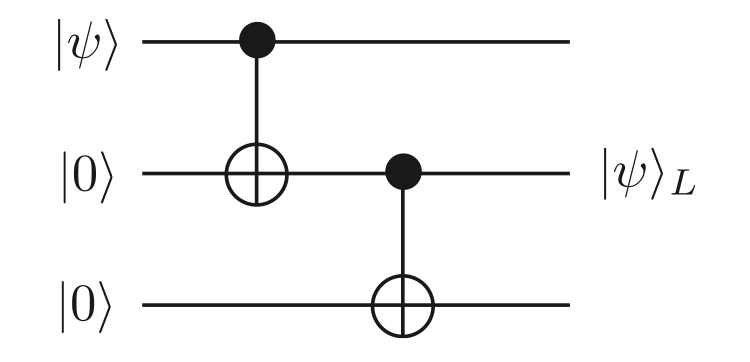
\includegraphics[width=0.5\linewidth]{images/error-correction/Abb1_BitFlipCode_1.png}
  
  \vspace{1.2em} % Abstand zwischen den Bildern
  
  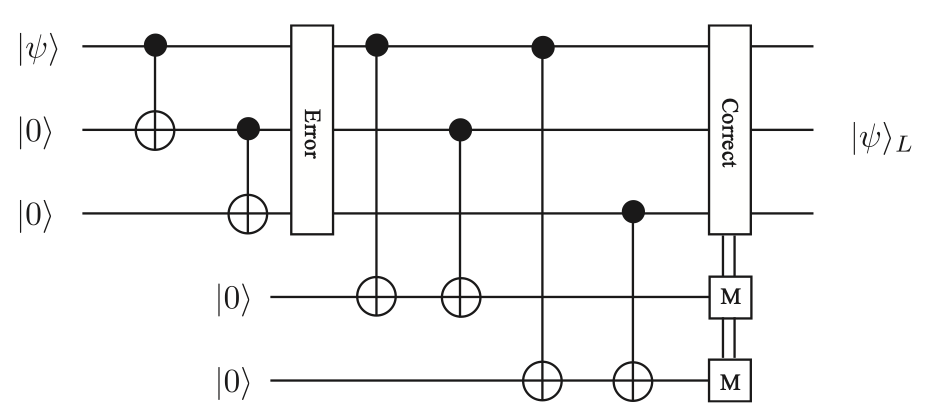
\includegraphics[width=0.75\linewidth]{images/error-correction/Abb2_BitFlipCode_2.png}
  
  \caption{Kodierung eines logischen Qubits in drei physikalische Qubits mittels CNOT-Gattern (3-Qubit-Bitflip-Code). Unten: Gesamter Zyklus aus Kodierung, Fehler, Syndrommessung und Korrektur auf Basis desselben Codes (vgl.~\cite[8]{devitt_quantum_2013}).}
  \label{fig:bitflipcode}
\end{figure}

Die Funktionsweise des 3-Qubit-Bitflip-Codes ist in Abbildung~\ref{fig:bitflipcode} dargestellt.
Der obere Teil zeigt die Kodierung eines logischen Qubits auf drei physikalische Qubits mit Hilfe von CNOT-Gattern.
Darunter ist der vollständige Fehlerkorrekturzyklus schematisch zusammengefasst: von der Kodierung über die Fehlererkennung (Syndrommessung) bis zur gezielten Korrektur (vgl.~\cite[8]{devitt_quantum_2013}).
\medskip
\paragraph{3-Qubit-Wiederholungscode (Phasenflip-Code):}\label{chap:QEC1.4}

Wie in Abschnitt~\ref{chap:QEC1.3} beschrieben, wirkt ein Phasenfehler durch Anwendung des Pauli-\(Z\)-Operators auf einen Qubit-Zustand. Dabei bleibt \(|0\rangle\) unverändert, während \(|1\rangle\) in \(-|1\rangle\) übergeht:
\[
Z(a|0\rangle + b|1\rangle) = a|0\rangle - b|1\rangle
\]
Ein solcher Vorzeichenwechsel ist in der Standardbasis \(\{|0\rangle, |1\rangle\}\) nicht direkt messbar. Betrachtet man jedoch den Zustand in der sogenannten \emph{Hadamard-Basis}, also in der Basis \(\{|+\rangle, |-\rangle\}\) mit
\[
|+\rangle = \frac{1}{\sqrt{2}}(|0\rangle + |1\rangle), \quad |-\rangle = \frac{1}{\sqrt{2}}(|0\rangle - |1\rangle),
\]
so wirkt der Phasenfehler wie ein klassischer Bitflip:
\[
Z|+\rangle = |-\rangle, \quad Z|-\rangle = |+\rangle
\]
Diesen Zusammenhang macht man sich zunutze, indem man einen Bitflip-Code in der Hadamard-Basis anwendet. Die logischen Zustände des Phasenflip-Codes lauten:
\[
|0_L\rangle = |+++\rangle, \quad |1_L\rangle = |---\rangle
\]
Ein einzelner Phasenfehler auf einem der drei Qubits kehrt den lokalen Zustand von \(|+\rangle\) zu \(|-\rangle\) um (oder umgekehrt), wodurch mithilfe von Paritätsmessungen (Syndromen) analog zum klassischen Wiederholungscode erkannt werden kann, welches Qubit betroffen ist. Eine anschließende \(Z\)-Operation korrigiert den Fehler, ohne die Superposition zu zerstören (vgl.~\cite[430-431]{nielsen_quantum_2010} \cite[4]{devitt_quantum_2013}).
\medskip
\paragraph{Shor-Code (9-Qubit-Code):}

Peter Shor entwickelte 1995 den ersten Quantenfehlerkorrekturcode, der in der Lage ist, beliebige Ein-Qubit-Fehler zu korrigieren – also sowohl Bit-Flips (\(X\)), Phasen-Flips (\(Z\)) als auch Kombinationen davon (\(Y = iXZ\)). Der sogenannte Shor-Code kombiniert zwei einfache Schutzprinzipien: eines gegen Bitfehler und eines gegen Phasenfehler.

Das Grundprinzip besteht darin, ein einzelnes logisches Qubit auf \textbf{neun physikalische Qubits} zu verteilen. Dazu wird zunächst ein \textbf{Bit-Flip-Code} angewendet, der das Qubit dreifach wiederholt: \( |\psi\rangle \mapsto |\psi\rangle |\psi\rangle |\psi\rangle \). Das schützt gegen Bitfehler, also versehentliches Umdrehen von 0 zu 1 oder umgekehrt.
Anschließend wird jeder dieser drei Pfade durch ein \textbf{Hadamard-Gatter (\(H\))} in eine Superposition überführt. Danach folgt erneut eine dreifache Wiederholung – diesmal entlang der Zeilen. So entsteht ein Zustand, der gleichzeitig vor Phasenflips schützt (vgl.~\cite[10-11]{devitt_quantum_2013}).
In Abbildung~\ref{fig:shor_preparation} wird das Codieren der physischen Qubits auf ein logisches Qubit dargestellt.

\begin{figure}[htbp]
  \centering
  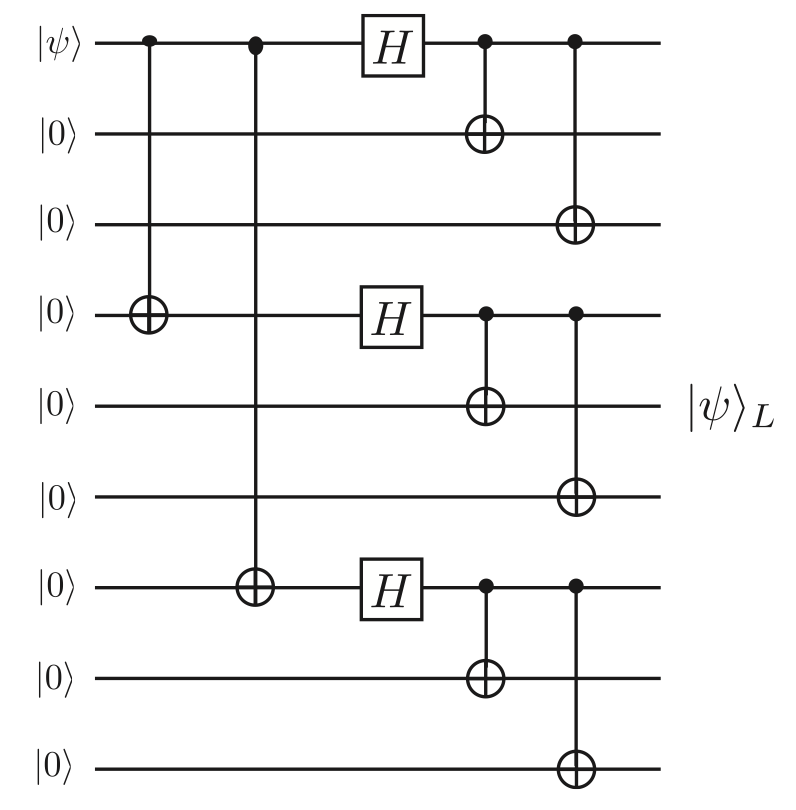
\includegraphics[width=0.75\linewidth]{images/error-correction/Abb3_ShorCode_1.png}
  \caption{Vorbereitung des Shor-Codes auf neun physikalischen Qubits. Zunächst erfolgt eine dreifache Wiederholung des Eingangszustands mithilfe von CNOT-Gattern. Anschließend wird auf jedem der drei Pfade ein Hadamard-Gatter \(H\) angewendet, das den Zustand in eine Superposition überführt. Danach folgt erneut eine dreifache Wiederholung (pro Zeile), um die Zustände \(|000\rangle \pm |111\rangle\) zu erzeugen (vgl.\ \cite[10]{devitt_quantum_2013}).}
  \label{fig:shor_preparation}
\end{figure}

Formal lassen sich die kodierten logischen Zustände wie folgt schreiben:
\[
\begin{aligned}
|0_L\rangle &= \frac{1}{\sqrt{8}} (|000\rangle + |111\rangle)(|000\rangle + |111\rangle)(|000\rangle + |111\rangle) \\
|1_L\rangle &= \frac{1}{\sqrt{8}} (|000\rangle - |111\rangle)(|000\rangle - |111\rangle)(|000\rangle - |111\rangle)
\end{aligned}
\]
vgl.~\cite[10]{devitt_quantum_2013}

Die Struktur ist dabei wie folgt aufgebaut: Jeder der drei Blöcke (je drei Qubits) bildet eine Superposition aus \(|000\rangle\) und \(|111\rangle\). Diese Superposition ist entweder additiv (für \(|0_L\rangle\)) oder subtraktiv (für \(|1_L\rangle\)). Dadurch entsteht ein verschränkter Gesamtzustand, der sowohl Bit- als auch Phasenfehler sichtbar macht.
Fehlererkennung erfolgt durch Messung sogenannter \textbf{Stabilisatoren} – das sind spezielle Operatoren, die Auskunft darüber geben, ob und wo ein Fehler aufgetreten ist, ohne den gespeicherten Zustand direkt zu zerstören. So bewirkt etwa ein Phasenfehler in einem Block den Wechsel von \(|000\rangle + |111\rangle\) zu \(|000\rangle - |111\rangle\), was sich im Vorzeichen niederschlägt. Diese Änderung kann durch Syndrommessungen erkannt und der Fehler durch gezielte Anwendung eines Pauli-Operators (\(X\) oder \(Z\)) korrigiert werden (vgl.~\cite[432-433]{nielsen_quantum_2010}).

Da ein \(Y\)-Fehler eine Kombination von \(X\)- und \(Z\)-Fehler ist, genügt es, beide Einzelfehlerarten behandeln zu können. Der Shor-Code erfüllt diese Anforderung und besitzt die Parameter \([[9, 1, 3]]\): Er kodiert ein logisches Qubit in neun physikalische und kann bis zu zwei Fehler erkennen – sowie einen davon zuverlässig korrigieren (vgl.~\cite[10-11]{devitt_quantum_2013})

Auch wenn der Code praktisch aufwendig ist, markiert er einen Meilenstein der Quanteninformationsverarbeitung: Er bewies erstmals, dass sich Quanteninformation durch geschickte Kodierung und nicht-destruktive Messung grundsätzlich vor Fehlern schützen lässt (vgl.~\cite[Seite 432–434]{nielsen_quantum_2010})
\medskip
\paragraph{Steane-Code (7-Qubit-Code):}

Der 1996 von Andrew Steane entwickelte 7-Qubit-Code ist einer der bekanntesten Quantenfehlerkorrekturcodes. Er basiert auf einem klassischen Hamming-Code und gehört zur Familie der sogenannten CSS-Codes (Calderbank-Shor-Steane). Ziel ist es, Ein-Qubit-Fehler aller Art (Bitflips \(X\), Phasenflips \(Z\) und Kombinationen daraus) mit möglichst wenigen Qubits zu erkennen und zu korrigieren.

Der Steane-Code nutzt eine clevere Strategie: Er wählt bestimmte Bitmuster aus dem klassischen \([7,4,3]\)-Hamming-Code, die sich so stark voneinander unterscheiden, dass ein einzelner Fehler sie nicht ineinander überführen kann. Diese klassischen Wörter werden anschließend in eine Superposition überführt – so entsteht echte Quantenredundanz.

Die beiden logischen Zustände \(|0_L\rangle\) und \(|1_L\rangle\) bestehen jeweils aus einer Superposition von acht solchen 7-Bit-Wörtern. Alle ausgewählten Bitmuster erfüllen spezielle Paritätsbedingungen, die es erlauben, auftretende Fehler mit sogenannten Stabilizer-Messungen zu identifizieren und zu korrigieren:
\[
\begin{aligned}
|0_L\rangle &= \frac{1}{\sqrt{8}} \big( 
|0000000\rangle + |1010101\rangle + |0110011\rangle + |1100110\rangle + {} \\
&\quad |0001111\rangle + |1011010\rangle + |0111100\rangle + |1101001\rangle \big) \\
|1_L\rangle &= \frac{1}{\sqrt{8}} \big( 
|1111111\rangle + |0101010\rangle + |1001100\rangle + |0011001\rangle + {} \\
&\quad |1110000\rangle + |0100101\rangle + |1000011\rangle + |0010110\rangle \big)
\end{aligned}
\]

Durch diese Struktur lässt sich mit nur sieben Qubits ein vollständiger Schutz gegen Ein-Qubit-Fehler erreichen – genau wie beim Shor-Code, aber effizienter.
Die Zustände \(|0_L\rangle\) und \(|1_L\rangle\) bestehen aus Superpositionen scheinbar willkürlicher Bitmuster wie \(|1010101\rangle\) oder \(|1100110\rangle\). Tatsächlich sind diese Muster jedoch gezielt gewählt:

\begin{itemize}
  \item Sie stammen aus dem klassischen \([7,4,3]\)-Hamming-Code, der bekannte Fehlerkorrektureigenschaften hat.
  \item Die Bitfolgen erfüllen bestimmte Paritätsbedingungen und sind so konstruiert, dass man bei einem einzelnen Bitflip noch erkennen kann, welches Bit betroffen ist.
  \item Durch die Überlagerung mehrerer solcher gültiger Codewörter (Superposition) entsteht ein Quantenfehlerkorrekturcode, der sowohl Bit- als auch Phasenfehler erkennen kann.
\end{itemize}
Diese scheinbar komplizierten Muster sind also notwendig, um mit nur sieben Qubits vollständige Ein-Qubit-Fehlerkorrektur zu ermöglichen (vgl.~\cite[12]{devitt_quantum_2013}).
\medskip
\paragraph{Ausblick auf fortgeschrittene Codes:}

Die bisher vorgestellten Codes – wie der Drei-Qubit-Code, der Shor-Code und der Steane-Code – zeigen, wie sich einzelne Bit- oder Phasenfehler gezielt erkennen und korrigieren lassen. Während sie bereits vollständige Quantenfehlerkorrektur auf einem logischen Qubit ermöglichen, stoßen sie bei wachsender Qubit-Anzahl und praktischer Realisierung an ihre Grenzen.

Für den Aufbau skalierbarer Quantencomputer werden daher weiterentwickelte Codefamilien benötigt, die neben der Korrektur beliebiger Fehler auch architektonische Vorteile bieten – etwa durch lokale Wechselwirkungen und effiziente Layouts. Ein prominentes Beispiel dafür sind die Oberflächencodes, die im folgenden Abschnitt behandelt werden. Sie beruhen auf denselben Grundprinzipien, setzen jedoch auf topologische Strukturen und fehlertolerante Operationen im Gitter.

\subsection{Der Fehlerkorrekturzyklus am Beispiel von Oberflächencodes}\label{chap:QEC3.2}

Der Oberflächencode basiert auf einem zweidimensionalen Gitter aus physikalischen Qubits, typischerweise in Form eines rechteckigen Flächenstücks (\emph{Patch}). Dabei unterscheidet man zwei Arten von Qubits: \emph{Daten-Qubits}, welche die eigentliche logische Quanteninformation tragen, und \emph{Mess-Qubits}, die zur Fehlererkennung verwendet werden.

Man kann sich die Struktur wie ein Schachbrett vorstellen: Die Daten-Qubits liegen auf Kanten des Gitters, während die Mess-Qubits zwischen ihnen positioniert sind. Diese Mess-Qubits überwachen jeweils vier benachbarte Daten-Qubits. Dabei gibt es zwei Typen von Stabilizer-Operatoren:
\begin{itemize}
  \item \textbf{\(Z\)-Stabilizer} (auch \emph{Plaquette-Operatoren}\footnote{Plaquettes bezeichnen kleine quadratische Flächen im Gitter. Ein \(Z\)-Stabilizer wirkt auf die vier Daten-Qubits an den Ecken einer solchen Plaquette und erkennt Bitfehler.}) überprüfen die Parität in Bezug auf Bit-Flip-Fehler
  \item \textbf{\(X\)-Stabilizer} (auch \emph{Stern-Operatoren}\footnote{Stern-Operatoren wirken auf die vier Daten-Qubits, die an einem Gitterpunkt zusammenlaufen, und erkennen Phasenfehler.}) erkennen Phasenfehler
\end{itemize} (vgl.~\cite[676-679]{google_quantum_ai_suppressing_2023}).

\begin{figure}[htbp]
    \centering
    \includegraphics[width=0.6\linewidth]{images/error-correction/Abb4_Oberflaechencode_1.png}
    \caption{Stabilisatorstruktur eines 2D-Oberflächen-Codes. Gelbe Kreise repräsentieren Daten-Qubits. Graue Kreise stehen für Mess-Bits, die jeweils auf vier benachbarte Daten-Qubits wirken: Z-Stabilisatoren (blau) erkennen Bit-Flip-Fehler, X-Stabilisatoren (rot) erkennen Phasenfehler (vgl.~\cite{higgott_improved_2023}).}
    \label{fig:oberflaechencode-stabilisatoren}
\end{figure}

\paragraph{Syndrommessung und Fehlererkennung:}

Die Fehlerkorrektur erfolgt zyklisch. In jedem Zyklus werden alle \(X\)- und \(Z\)-Stabilizer gemessen. Dazu wird jedes Mess-Qubit mit den vier zugehörigen Daten-Qubits durch eine Reihe kontrollierter Gatter verschränkt, z.\,B. mit CNOT-Operationen. Nach dieser Verschaltung enthält das Mess-Qubit die Paritätsinformation: Bei \(Z\)-Stabilizern etwa, ob eine gerade oder ungerade Anzahl von \( |1\rangle \)-Zuständen in der Gruppe vorliegt. Anschließend wird das Mess-Qubit gemessen – in der \(Z\)-Basis für \(Z\)-Stabilizer und in der \(X\)-Basis für \(X\)-Stabilizer.

Das Ergebnis der Messung – 0 (Eigenwert \(+1\)) oder 1 (Eigenwert \(-1\)) – wird als \emph{Syndrom-Bit} bezeichnet. Es zeigt an, ob sich seit der letzten Messung ein Fehler ereignet hat. Wichtig ist: Diese Messungen beeinflussen den logischen Zustand nicht. Sie liefern nur Informationen über potenzielle Fehler, ohne die kodierte Quanteninformation direkt zu zerstören (vgl.~\cite[5-6]{fowler_surface_2012}).
\medskip
\paragraph{Decodierung und Fehlerlokalisierung:}

Die Menge aller Syndrom-Bits ergibt ein \emph{Syndrommuster}, aus dem auf die wahrscheinlichsten Fehler geschlossen werden kann. Ein einzelner Bitfehler an einem Daten-Qubit führt typischerweise dazu, dass zwei benachbarte \(Z\)-Stabilizer von 0 auf 1 wechseln. Analog dazu führt ein Phasenfehler zu Abweichungen bei zwei benachbarten \(X\)-Stabilizern (vgl.~\cite[7]{fowler_surface_2012}).

Diese lokalen Muster bilden die Grundlage für die sogenannte \emph{Decodierung}: Ein Algorithmus analysiert die Verteilung der Fehlerhinweise und rekonstruiert den wahrscheinlichsten Fehlerpfad. Häufig wird dazu ein Graph aufgebaut, in dem Syndromabweichungen als Knoten erscheinen. Der Decoder sucht dann eine möglichst kurze Verbindung dieser Knoten – z.\,B. mithilfe eines Minimum-Weight-Perfect-Matching-Algorithmus (vgl.~\cite[10-11]{fowler_surface_2012}).

Da auch Messungen fehlerhaft sein können, betrachtet man oft mehrere Zyklen hintereinander und baut einen 3D-Graphen mit der Zeitachse als dritter Dimension. Inkonstistente Syndrome über die Zeit hinweg deuten dann auf Messfehler hin (vgl.~\cite[2]{wu_micro_2025}).
\medskip
\paragraph{Korrekturoperation:}

Nach der Decodierung steht eine Hypothese über die Art und Position der Fehler zur Verfügung. Man könnte nun direkt eine Pauli-Korrekturoperation auf das betroffene Qubit anwenden – etwa ein weiteres \(X\), um einen Bitflip rückgängig zu machen.

In der Praxis verwendet man häufig stattdessen ein sogenanntes \emph{Pauli-Frame}\footnote{Ein Pauli-Frame ist ein rein klassisches Register, in dem alle erkannten Fehler notiert werden. Die tatsächliche physische Korrektur wird dadurch vermieden und stattdessen bei der Interpretation der Messdaten berücksichtigt. So spart man potenziell fehleranfällige Operationen.}. Dabei wird die Fehlerinformation nicht physisch korrigiert, sondern nur logisch „mitgeführt“ und am Ende beim Auslesen berücksichtigt. Das spart Ressourcen und reduziert zusätzliche Fehlerquellen.

Nach Abschluss eines Fehlerkorrekturzyklus beginnt sofort der nächste – denn in einem realen Quantencomputer können ständig neue Fehler auftreten. Die kontinuierliche Wiederholung des Zyklus ermöglicht daher langfristig stabile und fehlertolerante Quanteninformation.
\medskip
\paragraph{Einfacher Überblick: So funktioniert ein Fehlerkorrekturzyklus im Oberflächencode}Damit ein Quantencomputer trotz fehleranfälliger Qubits zuverlässig funktioniert, wird in kurzen Abständen automatisch überprüft, ob Fehler aufgetreten sind. Der Ablauf sieht dabei so aus:

\begin{enumerate}
  \item \textbf{Start:}  
  Alle Qubits werden in bekannte Anfangszustände gebracht. Die sogenannten Mess-Qubits sind bereit, nach Fehlern zu suchen.

  \item \textbf{Fehlersuche:}  
  Die Mess-Qubits „fragen“ ihre Nachbarn (die Daten-Qubits), ob alles in Ordnung ist. Aus ihren Antworten entsteht ein Muster aus Nullen und Einsen – das sogenannte \emph{Syndrom}.

  \item \textbf{Auswertung:}  
  Ein klassischer Computer schaut sich das Syndrom an und erkennt daraus, wo wahrscheinlich ein Fehler passiert ist.

  \item \textbf{Reaktion:}  
  Der Computer entscheidet, ob und wie ein Fehler korrigiert werden muss. Oft merkt man sich den Fehler einfach und berücksichtigt ihn später automatisch.

  \item \textbf{Neustart:}  
  Der nächste Zyklus beginnt sofort. So werden ständig neue Fehler früh erkannt – auch während der Quantencomputer rechnet.
\end{enumerate}

\subsection{Aktuelle H\"urden und was die Zukunft bringt}\label{chap:QEC3.3}

Trotz erster erfolgreicher Implementierungen steht die Quantenfehlerkorrektur (QEC) noch am Anfang ihrer praktischen Nutzbarkeit. Der Weg zu einem fehlertoleranten Quantencomputer ist gepflastert mit technischen und konzeptionellen Herausforderungen. In diesem Abschnitt beleuchten wir die zentralen H\"urden und geben einen Ausblick auf vielversprechende Entwicklungen.
\medskip
\paragraph{Qubit-Qualit\"at und Fehlerschwellen} 
Ein zentrales Problem ist die Qualit\"at der physikalischen Qubits selbst. Quantenfehlerkorrektur wirkt nur, wenn die zugrunde liegenden Fehlerraten hinreichend niedrig sind. Theoretisch existiert eine Fehlerschwelle, unterhalb derer Redundanz die Zuverl\"assigkeit erh\"oht\footnote{Siehe das Threshold-Theorem in Abschnitt~\ref{chap:QEC2}}. Praktisch liegt diese Schwelle typischerweise bei Fehlerraten $\lesssim 10^{-3}$. Viele Architekturen, wie supraleitende Qubits oder Ionenfallen, erreichen in Labordemonstrationen bereits Zweiqubit-Gates mit Fehlerraten im niedrigen Promillebereich, was vielversprechend ist (vgl.~\cite{noauthor_quantinuum_2022}). Doch um lange Quantenalgorithmen (z.B. Faktorisierung mit Shor bei $n=2048$) fehlerfrei auszuf\"uhren, m\"ussen logische Qubits \emph{stundenlang} koh\"arent bleiben -- ein Ziel, das nur mit sehr stabilen physikalischen Qubits erreichbar ist (vgl.~\cite{gidney_how_2021}).
\medskip
\paragraph{Massiver Qubit-Overhead}
Der immense Ressourcenbedarf ist eine der größten Hürden der Fehlerkorrektur. 
Wie Fowler~\textit{et al.} aufzeigen, benötigt bereits ein einzelnes, 
ausreichend fehlertolerantes logisches Qubit eine Größenordnung von 
\emph{$10^3$ bis $10^4$ physikalischen Qubits}, abhängig von der Fehlerrate der Hardware. 
Für nützliche Anwendungen wie die Faktorisierung einer 2048-Bit-Zahl mit dem Shor-Algorithmus 
skaliert dieser Bedarf dramatisch: Die Autoren schätzen, dass dafür insgesamt 
\emph{rund eine Milliarde physikalischer Qubits} nötig wären.

Heutige Quantenprozessoren umfassen jedoch erst wenige Hundert bis einige Tausend Qubits, die Skalenlücke ist also noch immens. Zudem bringt jeder weitere Qubit rein 
ingenieurtechnische Herausforderungen mit sich: Komplexe Verkabelung, 
ständige Kalibrierung und das thermische Management müssen für jedes einzelne 
Qubit gewährleistet werden.
\medskip
\paragraph{Technische Limitierungen bei Kryogenik und Auslese}
Besonders supraleitende Systeme m\"ussen bei 10--20\,mK betrieben werden. Hier stoßen Forscher schnell an Grenzen: Die K\"uhlung gro\ss er Quantenprozessoren erfordert aufw\"andige Verd\"unnungsk\"uhler \emph{(dilution refrigerators)}, und die Zahl der nach innen f\"uhrenden Kabel wird schnell zum Flaschenhals.  Auch die Kontrolle \"uber klassische Elektronik ist herausfordernd: Steuereinheiten befinden sich oft au\ss erhalb des K\"uhlsystems und m\"ussen mit tausenden Kan\"alen kommunizieren -- ein thermisches und technisches Problem (vgl.~\cite[1]{krinner_engineering_2019}). Ans\"atze wie Cryo-CMOS (Steuerelektronik bei tiefen Temperaturen) werden intensiv erforscht (vgl.~\cite[13.5.1-13.5.2]{charbon_cryo-cmos_2016}).
\medskip
\paragraph{Dekodierung: Komplex und latenzkritisch}
Selbst wenn alle Syndromdaten vorliegen, ist die Decodierung (Fehlerdiagnose und Korrekturvorschlag) ein nichttriviales Problem. Bei QEC-Zyklen im Mikrosekundenbereich und Millionen von Qubits entstehen Datenraten im Bereich hunderter Terabyte pro Sekunde. Diese m\"ussen in Echtzeit verarbeitet werden, idealerweise mit Latenzen $<1\,\mu$s. Daher ben\"otigt man spezialisierte Hardware-Decoder und ausgekl\"ugelte Algorithmen wie Minimum Weight Matching (vg.~\cite[3-4]{wu_micro_2025}).
\medskip
\paragraph{Nicht-ideale Fehler und Modellabweichungen}
+Die meisten QEC-Codes beruhen auf idealisierten Fehlermodellen (z.B. unkorrelierte, Pauli-artige Fehler). In realen Systemen treten jedoch korrelierte Fehler, Kaskadeneffekte und Leakage auf, die nicht leicht mit bestehenden Codes zu behandeln sind. Solche Abweichungen senken die effektive Fehlerschwelle und machen eine robuste Fehlerkorrektur schwieriger (vgl.~\cite[312]{terhal_quantum_2015}).
\medskip
\paragraph{Ausblick und neue Ans\"atze}
Die Forschung reagiert mit vielf\"altigen Strategien:
\begin{itemize}
    \item \textbf{Hardwareverbesserung:} Längere Kohärenzzeiten, stabilere Qubits und besseres Materialdesign sind zentrale Entwicklungsziele (vgl.~\cite[309]{terhal_quantum_2015})
    \item \textbf{Topologische Qubits:} Systeme wie Majorana-Moden versprechen inhärente Fehlerresistenz, sind aber noch experimentell (vgl.~\cite[320]{terhal_quantum_2015})
    \item \textbf{Modulare Architekturen:} Mehrere kleine Qubit-Module könnten vernetzt werden, um skalierbare Systeme aufzubauen (vgl.~\cite[332-333]{terhal_quantum_2015}).
    \item \textbf{Neue Codes:} Quantum-LDPC-Codes (vgl.~\cite[342]{terhal_quantum_2015}) oder Color Codes (vgl.~\cite[327]{terhal_quantum_2015}) bieten bessere Raten und Flexibilität, sind aber schwerer umzusetzen.
    \item \textbf{Ko-Design:} Eine enge Verzahnung von Hardware, Software und Fehlermodellen ist notwendig, um das Gesamtsystem zu optimieren (vgl.~\cite[308]{terhal_quantum_2015}).
\end{itemize}

\paragraph{Fazit} 
Die Quantenfehlerkorrektur hat sich in den letzten Jahren von einem theoretischen Konzept zu einem praktischen Forschungsfeld mit greifbaren Fortschritten entwickelt. Dennoch sind viele zentrale Herausforderungen ungel\"ost. Die kommenden Jahre werden entscheidend sein, um aus den heutigen Demonstratoren robuste, fehlertolerante Quantencomputer zu formen. Dabei ist klar: Ohne QEC ist skalierbares Quantencomputing unm\"oglich -- mit ihr aber wird es eines Tages m\"oglich sein, Probleme zu l\"osen, die klassisch unzug\"anglich bleiben.

\section{Praxisbeispiel: Der Shor-Code als einfacher Quantenfehlerkorrekturcode}
Wie bereits im Verlauf der vorherigen Seiten aufgezeigt sind Maßnahmen zur Fehlerkorrektur in Quantensystemen unabdingbar, um sinnvolle, verlässliche und fehlerfreie Berechnungen durchzuführen und die Technik des Quantencomputings weiter zu skalieren.

Während die bisherigen Kapitel eine theoretische Einführung in Fehlertypen, deren Auswirkungen und Korrekturalgorithmen gegeben haben, zielt das folgende Kapitel darauf ab die vorher theoretisch eingeführten grundlegenden Fehler wie 
\begin{enumerate}
    \item Bitflip (Rotation um die X-Achse),
    \item Phasenflip (Rotation um die Z-Achse),
    \item Y-Flip (Rotation um die Y-Achse, also eine Kombination aus Bit- und Phasenflip)
\end{enumerate}
in einem konkreten Problemlösungssetup, dem Shor-Algorithmus auf Quantencomputern, aufzuzeigen und unter Zuhilfenahme der IBM Qiskit Library anschaulich darzustellen.
\medskip
Während im Test-Setup initial eine eigene Rauschfunktion verwendet wurde, wurde die Vorgehensweise im Verlauf angepasst und es wurde nur ein Phasen-Fehler anstelle einer komplexen Multi-Fehler-Rauschfunktion injiziert, da die Ergebnisse der Rauschfunktion erheblich schwerer zu interpretieren gewesen wären und den didaktischen Sinn dieses Kapitels verfehlen würde.
\medskip
Der Shor-Algorithmus darf generell nicht mit dem gleichnamigen Shor-Code verwechselt werden, der bereits vorgestellt wurde. Während der Shor-Code einen Korrekturalgorithmus darstellt, handelt es sich beim Shor-Algorithmus um einen bekannten Algorithmus zur Faktorisierung von Primzahlen.

Da das Ziel dieses Kapitels das Aufzeigen eines Praxisbeispiels ist, wird der Shor-Code unter Zuhilfenahme des Shor-Algorithmus und der Faktorisierung der Zahl N=15 als praktischer Use-Case erklärt.

\subsection{Praxisbeispiel Shor-Algorithmus}
Der Shor-Algorithmus ist ein Verfahren zur Berechnung von Primfaktoren sehr großer Zahlen und ist dazu in der Lage die Periode, die zur Bestimmung der Faktoren notwendig ist, \textbf{in polynomieller Zeit} zu finden.
Die Periode im Shor-Algorithmus ist definiert als

\begin{equation}
    a^r mod N = 1
\end{equation}

Sie transformiert das in Bit-Computern schwierige Faktorisierungsproblem in ein lösbares Periodenfindungsproblem, welches durch die zuvor erläuterten Quanten-Eigenschaften der Superposition ermöglicht wird.
Während die besten klassischen Verfahren (z.B. General Number Field Sieve) subexponentielle Komplexität besitzen, findet der Shor-Algorithmus die Periode in polynomieller Zeit. Ein immenser Zugewinn, welcher gleichzeitig bei nur einem einzigen Fehler versagen würde und eindrücklich die Notwendigkeit von Fehlerkorrektur aufzeigt.

Seine korrekte Ausführung erfordert somit nicht nur eine ausreichende Anzahl von Qubits, sondern auch eine hohe Gattertreue und stabile Kohärenzeigenschaften über viele Taktzyklen hinweg.

\subsection{Implementierung in IBM Qiskit}
\textbf{Q}uantum \textbf{I}nformation \textbf{S}cience Kit (kurz Qiskit) ist eine Software zur Visualisierung von Quantenschaltkreisen, zur Simulation von Quantencomputer-ähnlichen Umgebungen und zur Entwicklung und Ausführung von Quantenalgorithmen. Neben Simulationsoptionen bietet IBM, die Firma hinter der Software, auch Zugriff zu eigenen Quantencomputern an (vgl.~\cite{frank_zickert_how_2023}).

\subsubsection{Der Aufbau}
Zum Aufbau und zur Darstellung der Funktion des Shor-Codes wurde folgendes Beispiel-Setup implementiert:


Der Schaltkreis besteht aus zwei Qubit-Registern. Er zeigt die zentrale Komponente von Shor's Algorithmus zur Faktorisierung einer Zahl N. Konkret wird dadurch die Periode ausgerechnet, was als Prozess der
Quantum Phase Estimation (QPE) bezeichnet wird.

Das obere Register (Qubits q\_0 bis q\_3) dient als Zählerregister und wird zu Beginn durch sog. Hadamard-Gates in eine Überlagerung aller möglichen Zustände versetzt, um Werte parallel untersuchen zu können.

Das untere Register (Qubits q\_4 bis q\_7) ist das sogenannte Funktionsregister und enthält das Ergebnis des modularen Exponenzierens zur Bestimmung der Periode.

Anschließend folgen vier kontrollierte Operationen, die jeweils die Funktion $f$ realisieren. Diese Operationen sind als eigenständige Schaltkreise dargestellt und sind jeweils an eines der oberen Qubits gekoppelt. Sie führen die Funktion in Abhängigkeit vom Zustand des Zählerregisters aus. Diese kontrollierten modularen Berechnungen sorgen dafür, dass sich die gesuchte Periode als Phase in den Amplituden des Zählerregisters abbildet.

Um diese Phase messbar zu machen, wird im nächsten Schritt die sogenannte Inverse Quantum Fourier Transformation (iQFT) auf das Zählerregister angewendet. Diese dekodiert die phasenbehafteten Überlagerungszustände und überführt sie in ein auslesbares Interferenzmuster. Die anschließende Messung der oberen Qubits ergibt einen Bitstring, aus dem sich mithilfe klassischer Nachbearbeitung (z.B. Kettenbruchzerlegung) die Periode $r$ rekonstruieren lässt (vgl.~\cite{frank_zickert_how_2023}).
Die Annahme im hier vorgestellten Beispiel ist, dass sich in einem zur Berechnung verwendeten Qubits ein Fehler manifestiert hat, der den Algorithmus ohne Korrektur nutzlos machen würde.

\subsubsection{Der Shor-Code als Lösung}
Um ein einzelnes logisches Qubit in einem Quantencomputer gegen Fehler zu schützen, verwendet der Shor-Code insgesamt neun physikalische Qubits - so auch im Rahmen dieses Praxisbeispiels.

Zur Implementierung in Qiskit wurde darauf aufbauend folgender Versuchsaufbau eingesetzt:

\begin{figure}
    \centering
    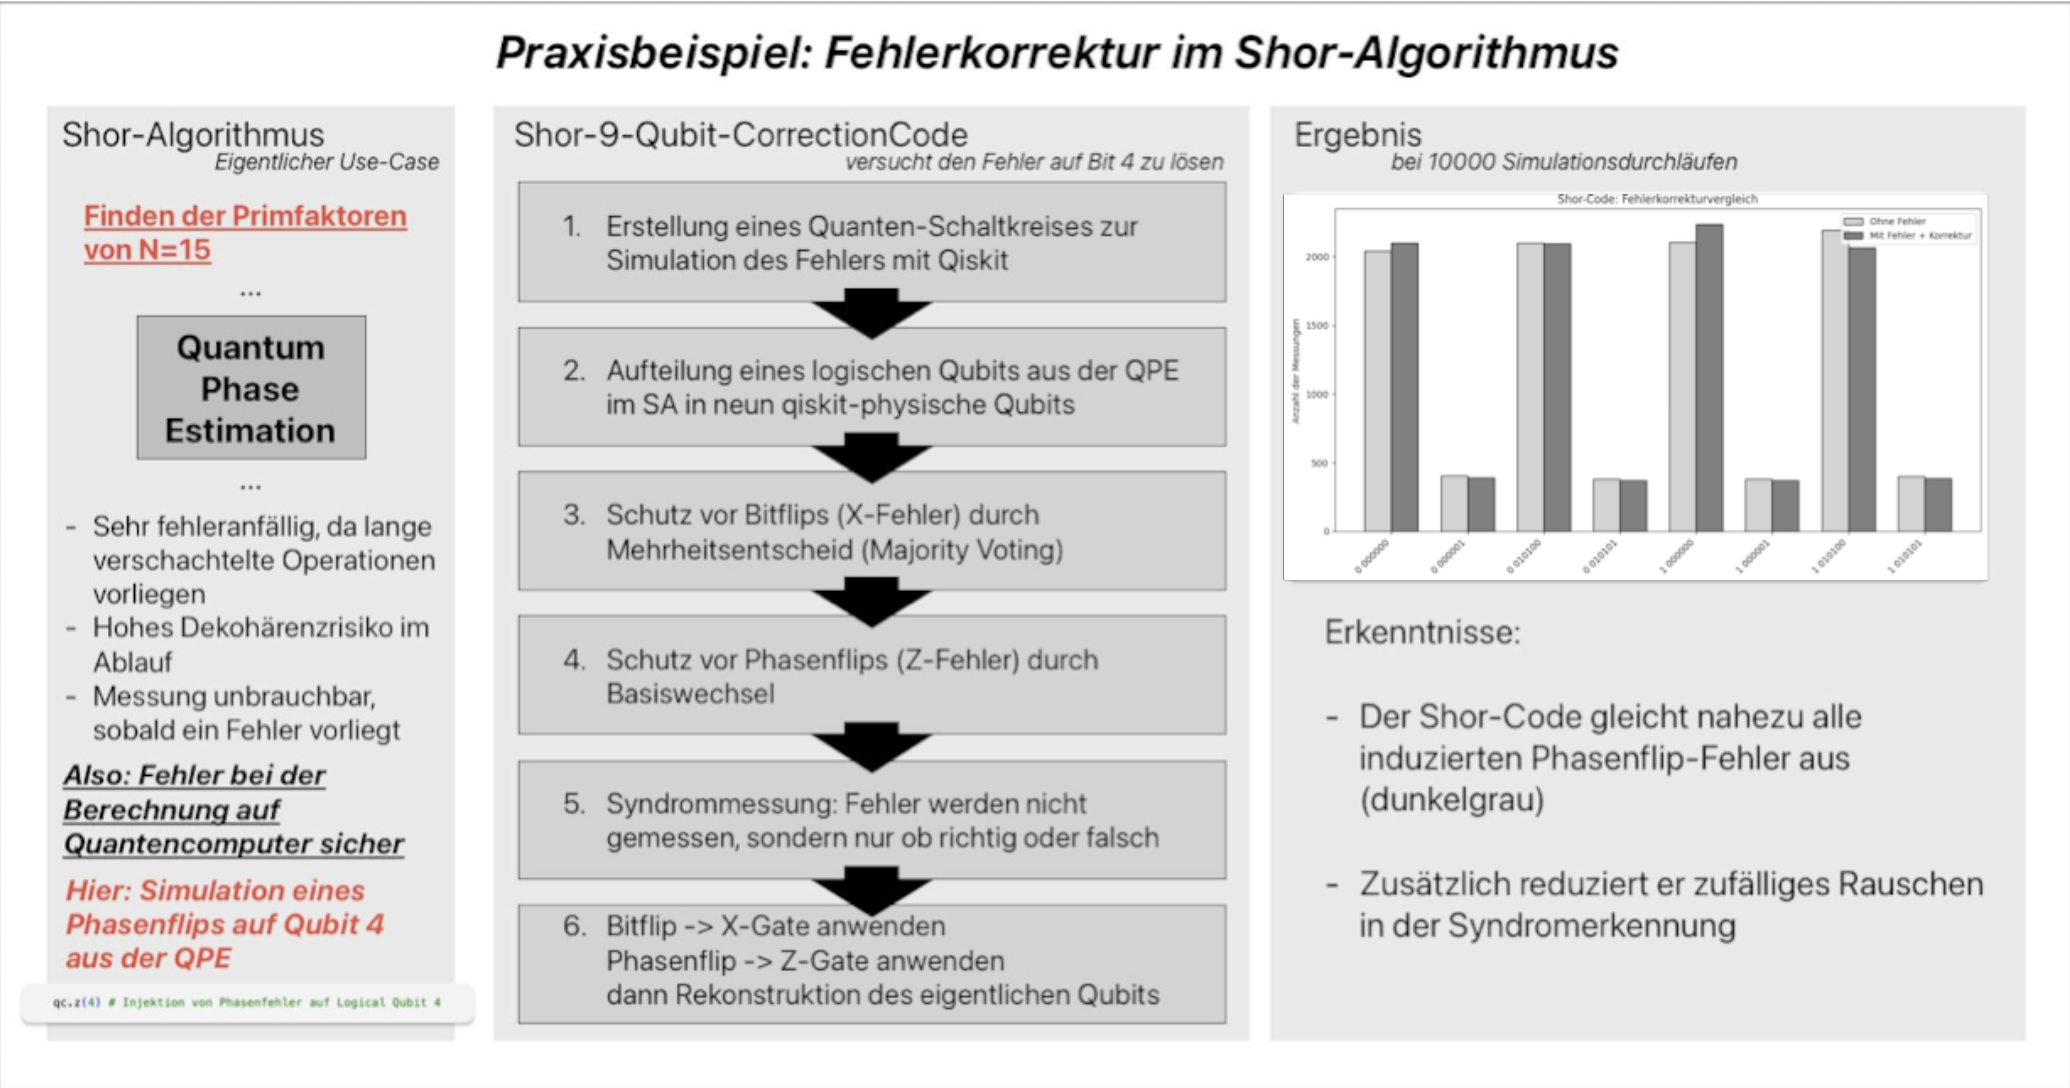
\includegraphics[width=1.0\linewidth]{images/praxis-example/study-design.png}
    \caption{Ausgehend vom initialen Use Case, der Anwendung des Shor-Algorithmus wurde der Shor-Code auf einen Phasenfehler angewendet.}
    \label{fig:study-design}
\end{figure}

\begin{enumerate}
    \item \textbf{Erstellung eines Quanten-Schaltkreises zur Simulation eines gezielten Fehlers mit Qiskit:} In einem Testaufbau wurde ein vereinfachter Shor-Algorithmus implementiert, bei dem der Fokus auf der Quantum Phase Estimation (QPE) lag. Um die Anfälligkeit des Verfahrens gegenüber Fehlern zu analysieren, wurde ein gezielter Phasenflip-Fehler auf \texttt{Qubit 4} (ein fiktives Qubit aus dem QPE-Register) induziert. Dies geschieht über den Befehl \texttt{qc.z(4)}.
\medskip
    \item \textbf{Aufteilung eines logischen Qubits in neun physische Qubits gemäß Shor-Code:} Zur Fehlerkorrektur wird das betroffene logische Qubit mithilfe der Shor-Kodierung in neun physikalische Qubits aufgeteilt. Dabei wird zuerst dreifach codiert (zum Schutz vor Bitflips) und anschließend jede dieser drei Kopien nochmals in der X-Basis dupliziert (zum Schutz vor Phasenflips laut Shor-Code). Diese redundante Kodierung ist essenziell für die spätere Fehlerdiagnose.
    \medskip
    \item \textbf{Schutz vor Bitflips durch Mehrheitsentscheid (Majority Voting):} Um X-Fehler zu erkennen, wird bei jeder Dreiergruppe von Qubits ein Mehrheitsentscheid getroffen: Wenn zwei der drei Qubits (also die Mehrheit) denselben Zustand haben, wird dieser als der ursprüngliche Zustand gewertet. Dies erlaubt die Korrektur einzelner Bitflips, ohne das logische Qubit zu zerstören.
\medskip
    \item \textbf{Schutz vor Phasenflips durch Basiswechsel:} Da Phasenfehler in der Z-Basis auftreten aber durch einen Wechsel in die X-Basis in Bitflip-Fehler transformiert werden können, wird jedes physische Qubit zusätzlich mit einem Hadamard-Gate (\texttt{H}) versehen. So wird der Schutzmechanismus gegen Bitflips indirekt auch zur Korrektur von Phasenflips eingesetzt.
\medskip
    \item \textbf{Syndrommessung:} Die Fehlererkennung erfolgt durch die Auswertung von sog. Syndromen. Diese zeigen nicht den exakten Fehler an, sondern liefern ein Muster, das angibt, ob ein Fehler vorliegt und an welcher Stelle er sich befinden könnte. Die eigentliche Information des logischen Qubits bleibt dabei erhalten, da es nicht gemessen wurde und sein Zustand somit nicht kollabiert ist.
\medskip
    \item \textbf{Fehlerkorrektur und Rekonstruktion:}  Wurde ein Bitflip festgestellt, wird es durch ein \texttt{X}-Gate korrigiert. Dasselbe gilt für Phasenfehler, die jedoch durch \texttt{Z}-Gates ersetzt werden. Nach der Korrektur wird das logische Qubit aus den physikalischen Qubits rekonstruiert und kann anschließend ausgelesen werden.
\end{enumerate}

In der Simulation wurden insgesamt \textbf{10\,000} Durchläufe durchgeführt. Die Ergebnisse zeigen, dass der Shor-Code nahezu alle gezielt induzierten Phasenflip-Fehler erfolgreich ausgleicht.


\subsubsection{Interpretation}
Das Ergebnis ist eindeutig: Die Auswertung zeigt, dass der Großteil der Fehler erfolgreich korrigiert werden konnte, was durch die gleichmäßige Verteilung der Balken für "mit Fehler + Korrektur" und "ohne Fehler" klar wird. 

\begin{figure}
    \centering
    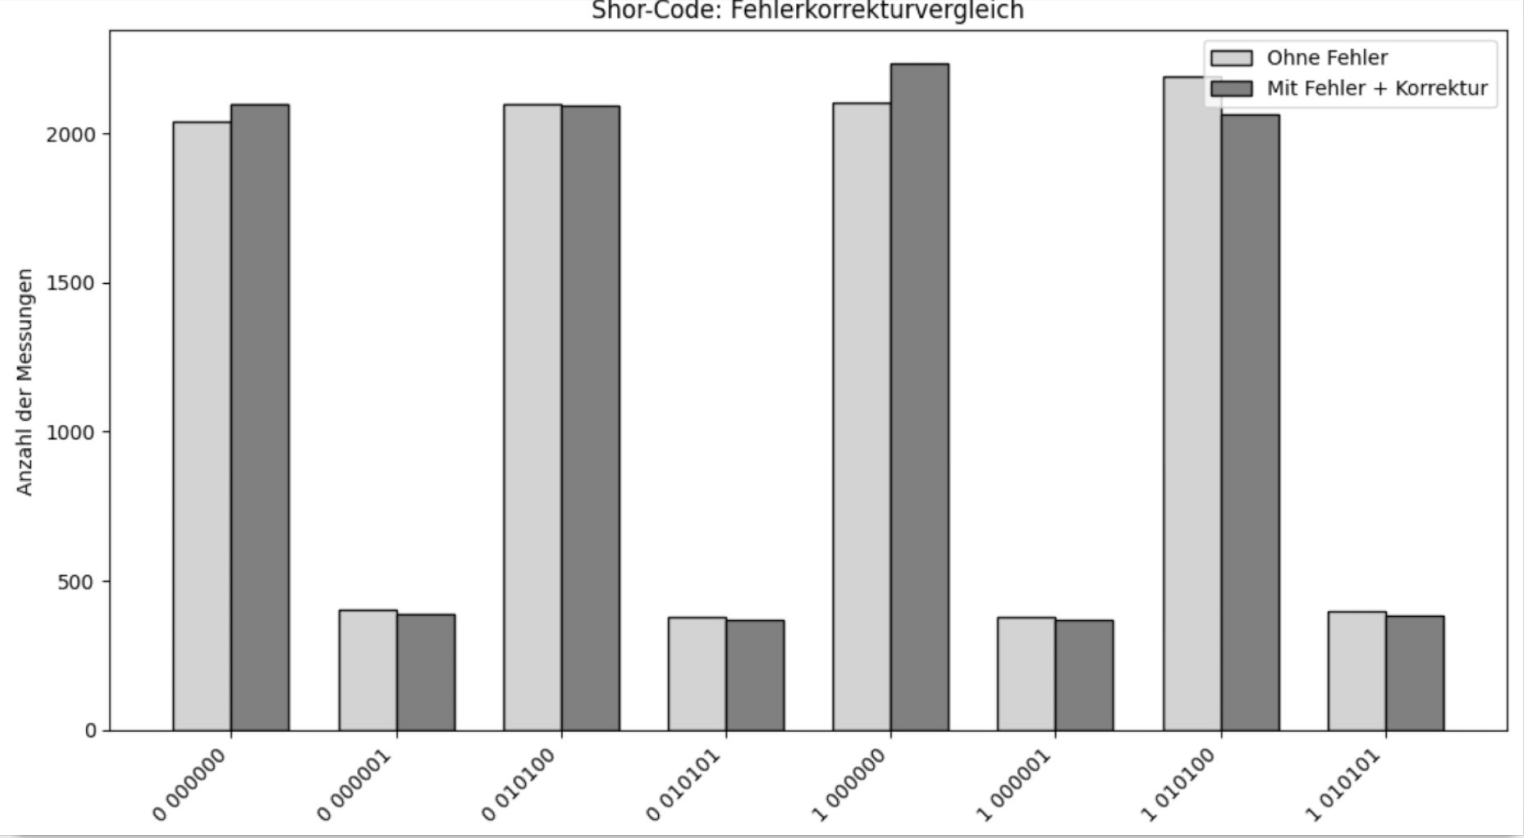
\includegraphics[width=0.8\linewidth]{images/praxis-example/error-distribution.png}
    \caption{Der Shor-Code erkennt den Großteil der induzierten Fehler und gleicht sie effizient aus.}
    \label{fig:error-dist}
\end{figure}
\noindent
\medskip
Die \textbf{Einordnung der Ergebnisse} geschieht folgendermaßen: 

Grundsätzlich lässt sich sagen, dass ein perfekter Zustand durch eine Gleichverteilung von "mit Fehler + Korrektur" und "ohne Fehler" erreicht werden würde, was aber in der Realität aufgrund von statistischen Ungenauigkeiten unrealistisch ist.

Die jeweils erste Ziffer der siebenstelligen Kombination repräsentiert das logische Qubit, und ist das Ergebnis aus der Rekonstruktion nach dem Prozess aus Majority Voting, Syndrommessung und Korrektur (Shor-Code Prozess).
Die sechs darauffolgenden Bits sind Syndrombits und repräsentieren die Messung der zuvor im Shor-Code definierten logischen Gruppen (Gruppe 1: Q0-2, Gruppe 2: Q3-5, Gruppe 3:Q6-8).
Jede dieser drei Gruppen gibt nun zwei Bits aus, die indizieren ob gruppen-intern ein Bit- oder einen Phasenflip (oder beides) vorliegt. Da im Test-Setup ein Phasen-Fehler auf Qubit 4 injiziert wurde, wird in keinem der Fälle ein Bit-Fehler festgestellt und die Fehler finden sich nur an den Stellen 2, 4 und 6 im rechten Syndromteil (bei den Phasen-Fehlern). 
Aufgrund der Funktionsweise des Shor-Codes wirken sich die Phasen-Fehler der zweiten Gruppe auch auf die Gruppen 1 und 3 aus. Für die Erkennung von Phasen-Fehlern wird auf alle Qubits kurz ein Hadamard-Gate angewandt, welches dann wieder zurück angewandt wird. Somit kann es zu übertragenden Fehlern kommen, die sich auch auf andere Gruppen auswirken.
Wichtig ist, dass es sich bei den Syndromen also nur um den Status bei der Messung handelt, nicht das finale Ergebnis. Die Korrektheit des Ergebnisses wird lediglich durch den dunkelgrauen Balken indiziert.
Syndrombits beschreiben also nur den Zustand vor der Korrektur, da die Phase der Syndrommessung im Prozess auch vor der eigentlichen Korrekutr stattfindet.

Davon ausgehend lassen sich folgende Aussagen über die ausgegebenen Syndrom-Strings treffen.

\begin{enumerate}
    \item \textbf{Balkenpaar: \texttt{0 000000}:} 
    Das erste Bit zeigt das logische Ergebnis 0, während alle Syndrombits den Wert 0 haben. 
    Auch in der Simulation mit injiziertem Fehler konnte der Fehler vollständig erkannt und korrigiert werden, sodass am Ende ein fehlerfreier Zustand gemessen wurde.

    \item \textbf{Balkenpaar: \texttt{0 000001}:}
    Im zweiten Balkenpaar nimmt das logische Qubit ebenfalls den Wert 0 an. Der Phasen-Fehler in Gruppe 3 ist auf die Verschränkung der Qubits als Teil des Shor-Codes und den damit einhergehenden Hadamard-Wechsel bei Phasen-Fehlern zurückzuführen. Dabei vermischt sich der Fehlerzustand und kann in den Messresultaten auch auf die Gruppe 3 wirken.

    
    \item \textbf{Balkenpaar: \texttt{0 010100}:}
    Auch bei Balkenpaar 3 wird das logische Qubit 0. Die Auswirkung auf die Gruppe 1 ist dabei dadurch zu erklären, dass die Fehlerkorrektur für Gruppe 2 erst nach der Syndromextraktion erfolgt und während der Extraktion alle Gruppen über ihre Hilfsqubits miteinander verschränkt sind.
    Dadurch kann ein in Gruppe 2 injizierter Fehler im endgültigen Syndromstring auch ein Phasen-Fehler in Gruppe 1 hervorrufen, ohne dass dort tatsächlich ein Fehler aufgetreten ist, da er auch nicht injiziert wurde und daher im perfekten (nicht beeinflussten) Zustand sein sollte.
    \item \textbf{Balkenpaar: \texttt{0 010101}:}
    Balkenpaar 4 kommt selten vor, da eine Ausprägung des Phasen-Fehlers auf alle drei Gruppen eher selten ist. Auch hier zeigt das Diagramm jedoch, dass die Fehler durch den Shor-Code ausgeglichen werden konnten.
    \item \textbf{Balkenpaare 5-8:} 
    Verhalten sich analog zu 1-4, mit dem Unterschied, dass das logische Qubit letztlich den Zustand 1 angenommen hat.
\end{enumerate}


Die aus dem Test-Setup abzuleitenden Resultate lassen mehrere Schlüsse zu:

\begin{itemize}
    \item Die Häufigkeiten der dominanten Ausgabewerte (\texttt{0 000000}, \texttt{1 000000}, \texttt{0 001010}, \texttt{1 001010}) bleiben trotz gezielt eingebrachten Fehlern und anschließender Korrektur größtenteils erhalten. Dies zeigt, dass das korrekte Messergebnis des logischen Qubits durch die Fehlerkorrektur \textbf{erfolgreich wiederhergestellt werden kann}, nachdem der Fehler auf Qubit 4 erzeugt wurde. Das gilt auch, wenn der Fehler im Prozess des Shor-Codes auf andere Gruppen übergesprungen ist.
    \medskip
    \item Die leichte Verschiebung einzelner Häufigkeiten (z.,B. \texttt{1 001010} von 2189 auf 2064) lässt sich möglicherweise durch Rauschen oder Unschärfen in der Syndrommessung erklären, beeinträchtigt jedoch die Wirkung der Fehlerkorrektur nicht signifikant.
\end{itemize}



\begin{table}[h!]
\centering
\begin{tabular}{|c|c|c|}
\hline
\textbf{Output-String} & \textbf{Ohne Fehler} & \textbf{Mit Fehler + Korrektur} \\
\hline
0 000000 & 2042 & 2101 \\
0 001010 & 2099 & 2092 \\
0 100000 & 405  & 387  \\
0 101010 & 379  & 368  \\
1 000000 & 2106 & 2234 \\
1 001010 & 2189 & 2064 \\
1 100000 & 380  & 370  \\
1 101010 & 400  & 384  \\
\hline
\end{tabular}
\caption{Vergleich der Messergebnisse mit und ohne Fehlerkorrektur}
\label{tab:shor_correction}
\end{table}



\subsubsection{Fazit}
Wie bereits in den vorangegangenen Kapiteln dargestellt, existieren heute deutlich modernere Verfahren zur Fehlerkorrektur in Quantenalgorithmen: etwa Surface-Codes, die eine höhere Fehlertoleranz aufweisen, allerdings auch mit einem deutlich größeren Ressourcenaufwand verbunden sind.
Nichtsdestotrotz stellt der hier untersuchte Shor-9-Qubit-Code einen anschaulichen didaktischen Einstieg in das Thema der Quantenfehlerkorrektur dar und kann als Grundlage für eine vertiefte Auseinandersetzung mit weiterführenden Methoden und komplexeren Algorithmen dienen.

\newpage
\printbibliography
